\chapter{Progress}
\section{Introduction}
In this chapter the data mining methods used to retrieve movement patterns from the TU Delft eduroam Wi-Fi log data will be described in detail. \autoref{workflow} gives an overview of the main workflow to derive movement patterns from the Wi-Fi log. First the raw data of the wifilogs are preprocessed to get states at two levels of detail (building- and building-part level). A state is defined as a time interval during which a particular device is located in a certain area. An example of a state on building level is: device A is located at Library from 11:00 to 12:00. An example on building part level is: device A is located at cantina from 11:00 to 12:00. These states are used to retrieve movements at both levels of detail. Movement is always from the location of one state to the location of another state. Furthermore, the building level states are used to retrieve trajectories and associate buildings with each other. The trajectories are defined for each person by an ordered list of buildings that were visited. Similarly a list of buildings is stored for each person for building association, however the order is neglected in this case. Finally, the movements on two levels of details, the trajectories and the associated buildings are all used to derive movement patterns.

In the following sections all these steps to derive different movement patterns are described in more detail. In \autoref{preprocessing} various pre-processing steps to clean, reduce and enrich the raw data will be discussed. Subsequently \autoref{movement between buildings} addresses the creation and visualization of movement on building level, this includes movement between buildings and movement from and to the campus.  \autoref{trajectories} and \autoref{Associated buildings} cover trajectories and building association respectively. \autoref{entrances and exists} and \autoref{Static and mobile devices} on entrances and static vs mobile are not implemented in the main workflow yet as the work is still in the exploratory phase. Finally \autoref{results} gives an overview of all the preliminary results.

\begin{figure}[H]
\centering
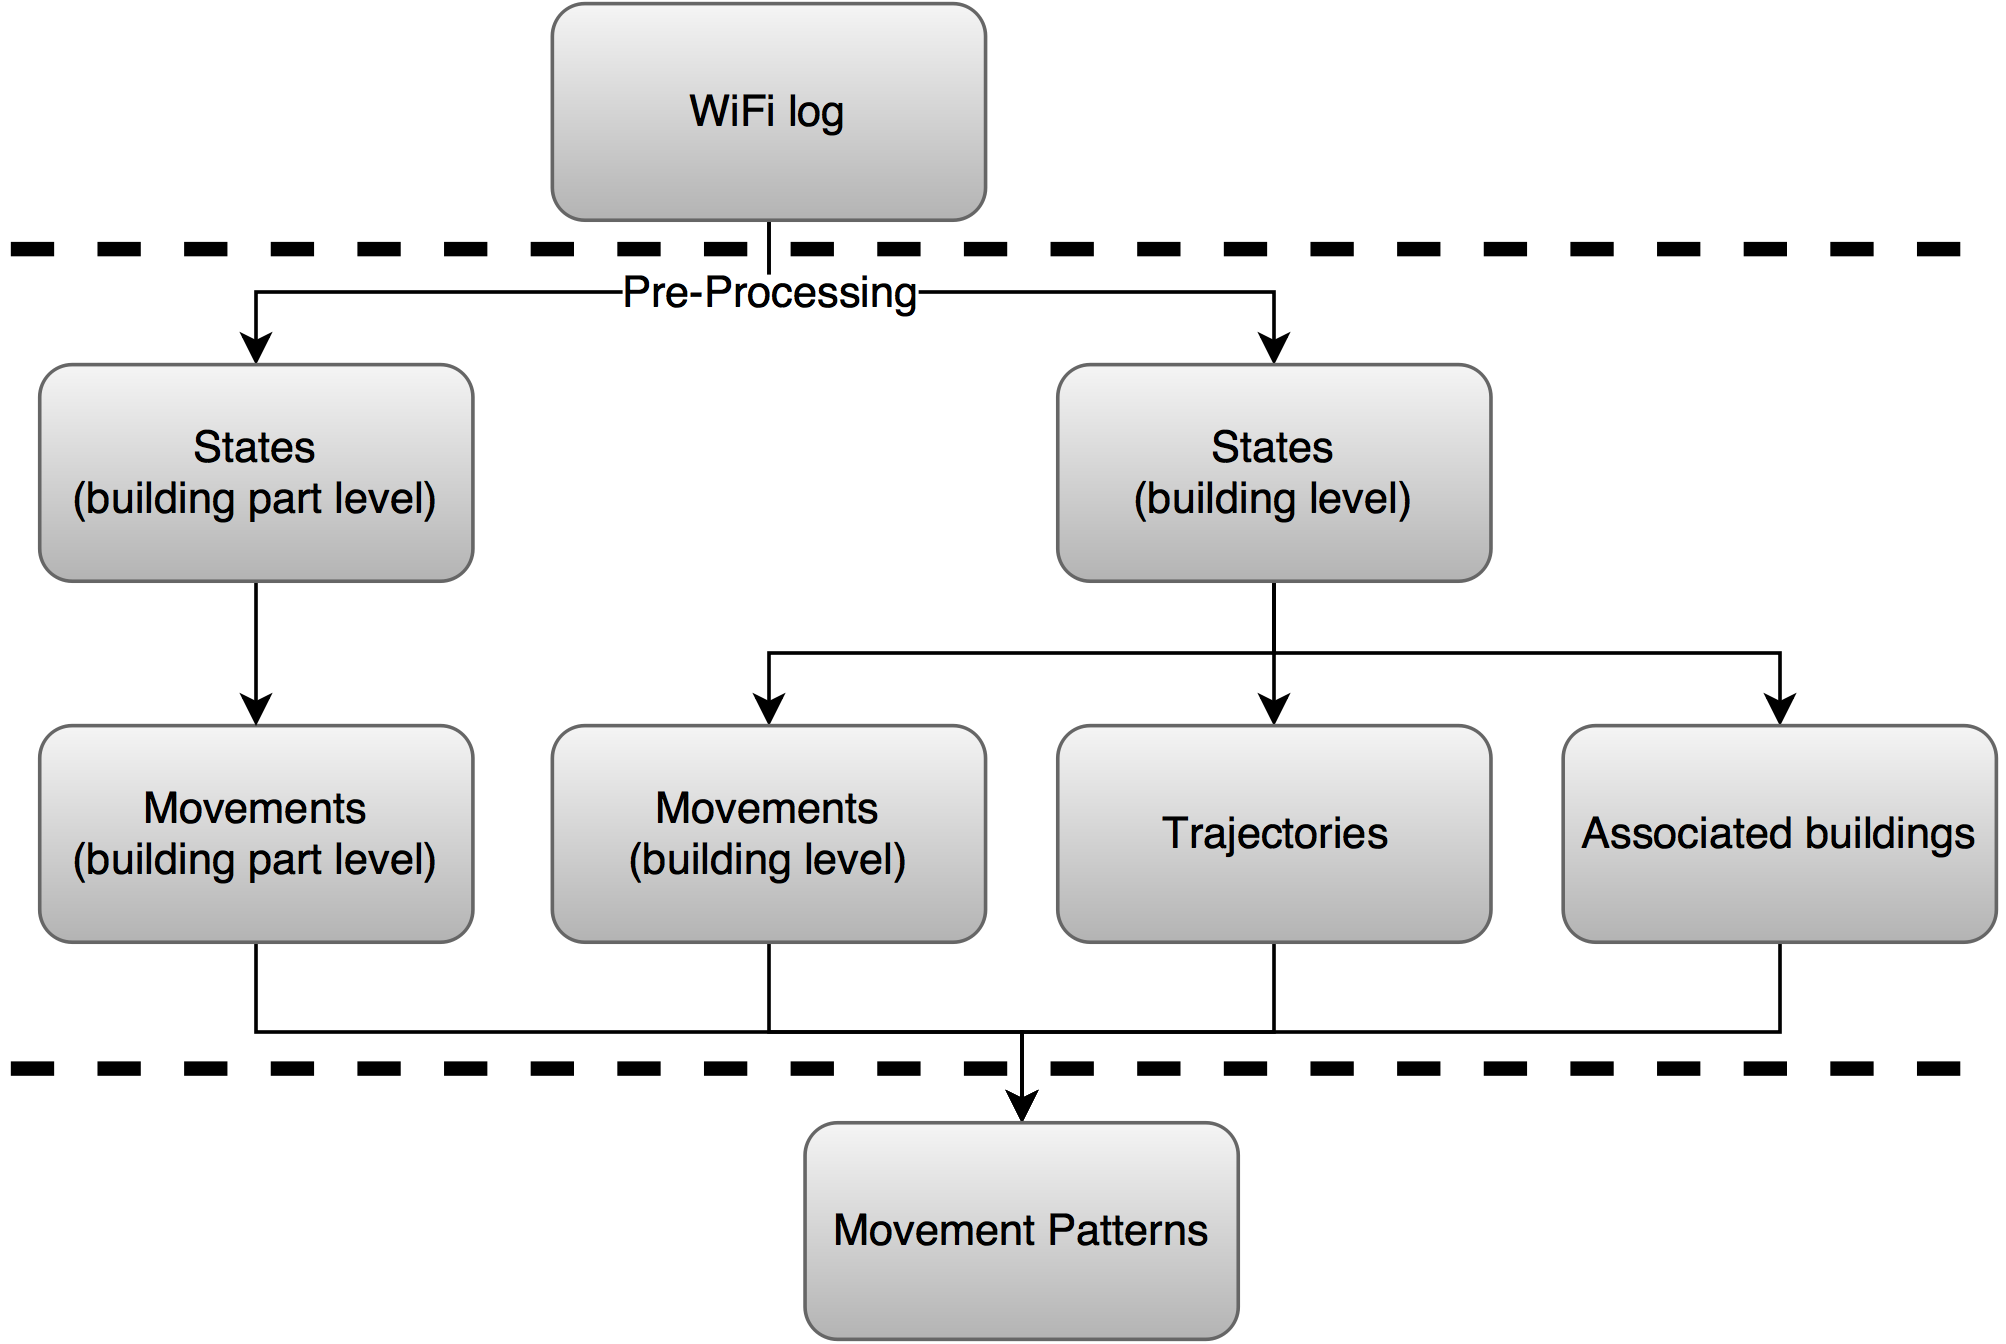
\includegraphics[scale=0.2]{methods.png}
\captionsetup{justification=centering}
\caption{Methods}
\label{workflow}
\end{figure}

\section{Pre-Processing}\label{preprocessing}
Before movement patterns between buildings can be retrieved, pre-processing of the raw data is required. In this chapter the different pre-processing steps will be described in detail. First \autoref{generalfiltering} addresses the initial data filtering. \autoref{filling} describes the filling of the dataset with a 'world' location, this enables detection of movement from and to the campus..\autoref{filtering} is about filtering of records of people only passing by a building. Finally \autoref{grouping} concerns the grouping of records of the same mac address that are subsequent in time and at the same location.
\subsection{General filtering}\label{generalfiltering}
Each record in the wifilog represents the scanning of a certain device at a certain time by a certain access point. In order to detect the movement patterns of these devices between buildings it should be known for each access point in which building it is located. The apname field in the wifilog table includes the building id in which building each scanner is located. However for some access points the apname is given in a different format and as a result their location is unknown. These apnames have in common that they don’t contain the '-' character which is present in all the other apnames. As a result the apnames of which the location is not known can simply be filtered out by checking if a '-' is present in the apname. 

\subsection{Filling}\label{filling}
Because the dataset contains all records of when certain devices are scanned, it also Implicitly stores information on when the device is not located at the campus. These time gaps in which a particular device is not scanned at the campus give information on when the corresponding person is not at the campus. This information is valuable for detecting movement patterns from and to the campus in addition to the movement between buildings at the campus. Considering the fact that many student only visit one faculty each day. It becomes especially clear, that the movement from and to the campus plays an important role in the overall movement pattern of a person. In order to be able to directly derive movement from and to the campus from the dataset, the time gaps present in the data should be stored explicitly. Therefore each time gap larger than an hour is filled with a 'world' record. The word 'world' is used to indicate that the device could be located at any place in the world during the time spans that it is not scanned at the campus. The begin and end time of a world record is defined by the end of the previous record and the start of the next record in time. In case there is no previous or next record the boundaries are defined by the starting time of the whole dataset and the current time. \autoref{figure:filling} visualizes the filling of time gaps for one devices. The black intervals indicate the time during which a device was scanned at the campus, the red intervals indicate the time gaps filled with a world records. Note that the gap at 16:00  is smaller than an hour and therefore is not filled.
\begin{figure}[H]
\centering
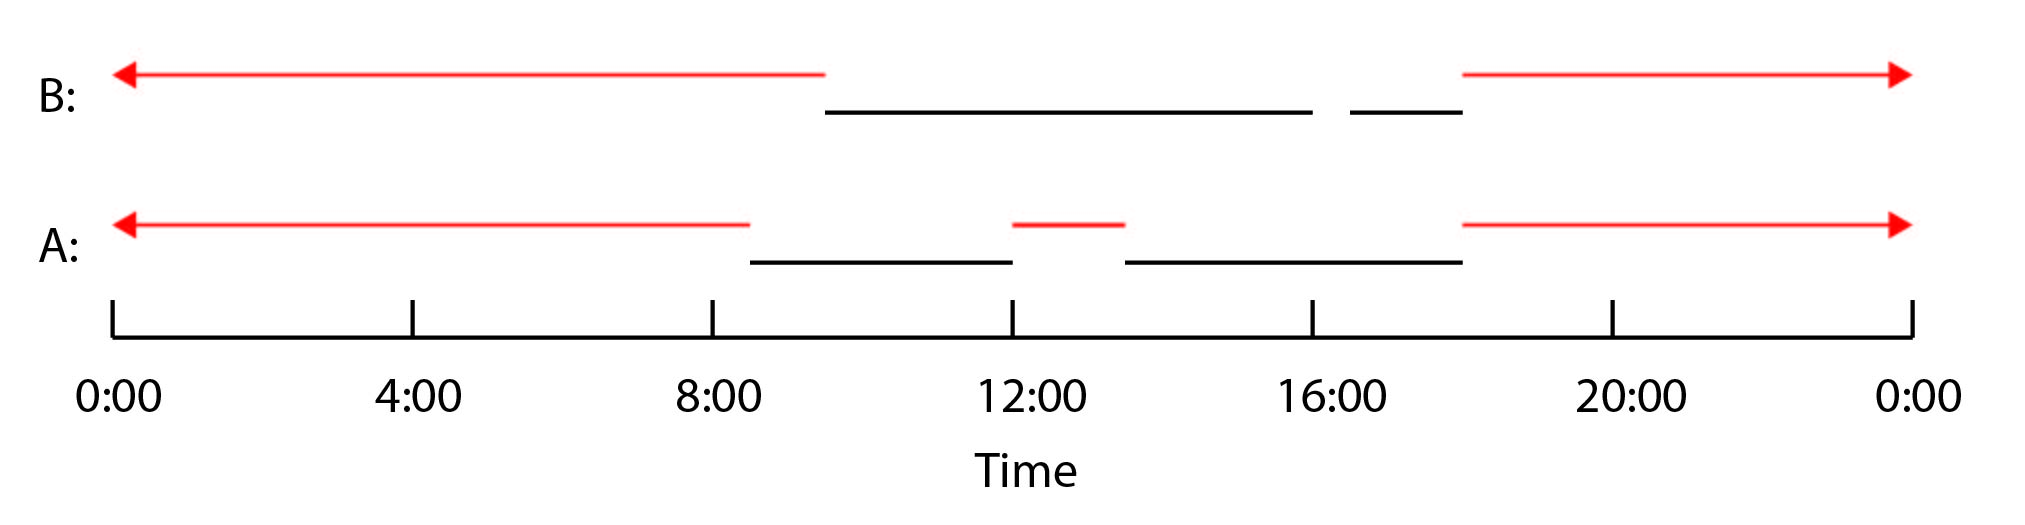
\includegraphics[scale=0.2]{Filling-01}
\captionsetup{justification=centering}
\caption{Filling}
\label{figure:filling}
\end{figure}

\subsection{Grouping}\label{grouping}
In order to reduce the data and to be able to filter on people only passing by a building without going in, the data needs to be grouped. The goal is to identify movement patterns between different buildings, this means that records of subsequent scans of the same device in the same building can be grouped together into one single record. The mobile of someone who for example studies the whole day at architecture might have 20 records in the database for that day. This can be reduced to one record that states the time the device arrived at Architecture and left again. To determine whether two records are subsequent in time, and therefore should be grouped together, a threshold for the time gap between two records needs to be defined. As explained in section … the eduroam system has 'scanning rounds' at intervals of 5 minutes and several seconds. If a device is not scanned during a scannig round, but was scanned the round before, the end time of the records is set to the time of the previous scan round plus 5 minutes (see record A1 and B1 \autoref{figure:grouping}). As a result the gap will be a bit more than 10 minutes if someone is not scanned for 2 subsequent rounds (\autoref{figure:grouping} A), and a bit more than 15 minutes if someone is not scanned for 3 subsequent rounds (\autoref{figure:grouping} B). It was decided to set the gap threshold or grouping to 15 minutes. The reasoning behind this is that someone who is not scanned for 3 subsequent rounds has likely left the building. For the example this means records A1 and A2 would be grouped together, records B1 and B2 on the other hand are not grouped.

\begin{figure}[H]
\centering
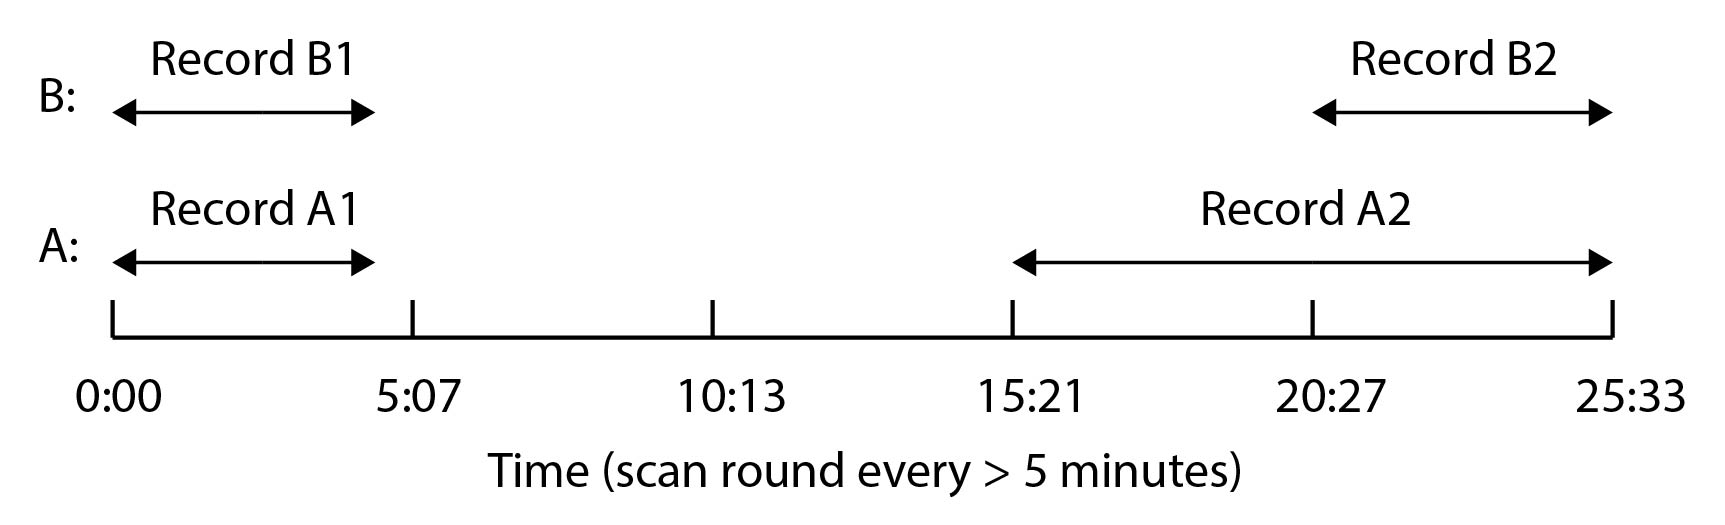
\includegraphics[scale=0.2]{grouping-01}
\captionsetup{justification=centering}
\caption{Grouping}
\label{figure:grouping}
\end{figure}

\subsection{Filtering}\label{filtering}

For the detection of movement patterns between buildings, records of people that only pass by a building without actually visiting it should be excluded. The reason for this is that records of people only passing by a building could result in misinterpretation of the movement patterns. If faculty B is for example located on the route from faculty A to the lunch facility. Then it is likely that people moving from faculty A to the lunch facility are picked up by a scanner located at faculty B. As a result the movement from faculty A to the lunch facility will be visualized via faculty B (see \autoref{figure:passing by} top). Someone that isn’t aware of the 'passing by' problem might conclude that people from faculty B make most use of the lunch facility. In reality however, people from faculty A make more use of the lunch facility. By filtering out the records of people only passing by buildings the correct movement can be visualized (see \autoref{figure:passing by} bottom). It should be noted that filtering out 'passing by' records can only be done after the grouping process. The reason for this is that 5-minute records that would individually be classified as someone passing by might be grouped together. After grouping the combined record is not classified as someone who passes by. Furthermore it should be noted that the filtering of 'passing by' records occurs after filling the data with 'world' records. The reason for this that a passing by event does mean that the device was located on the campus. The world records are meant to represent the time the device is not on the campus.

\begin{figure}[H]
\centering
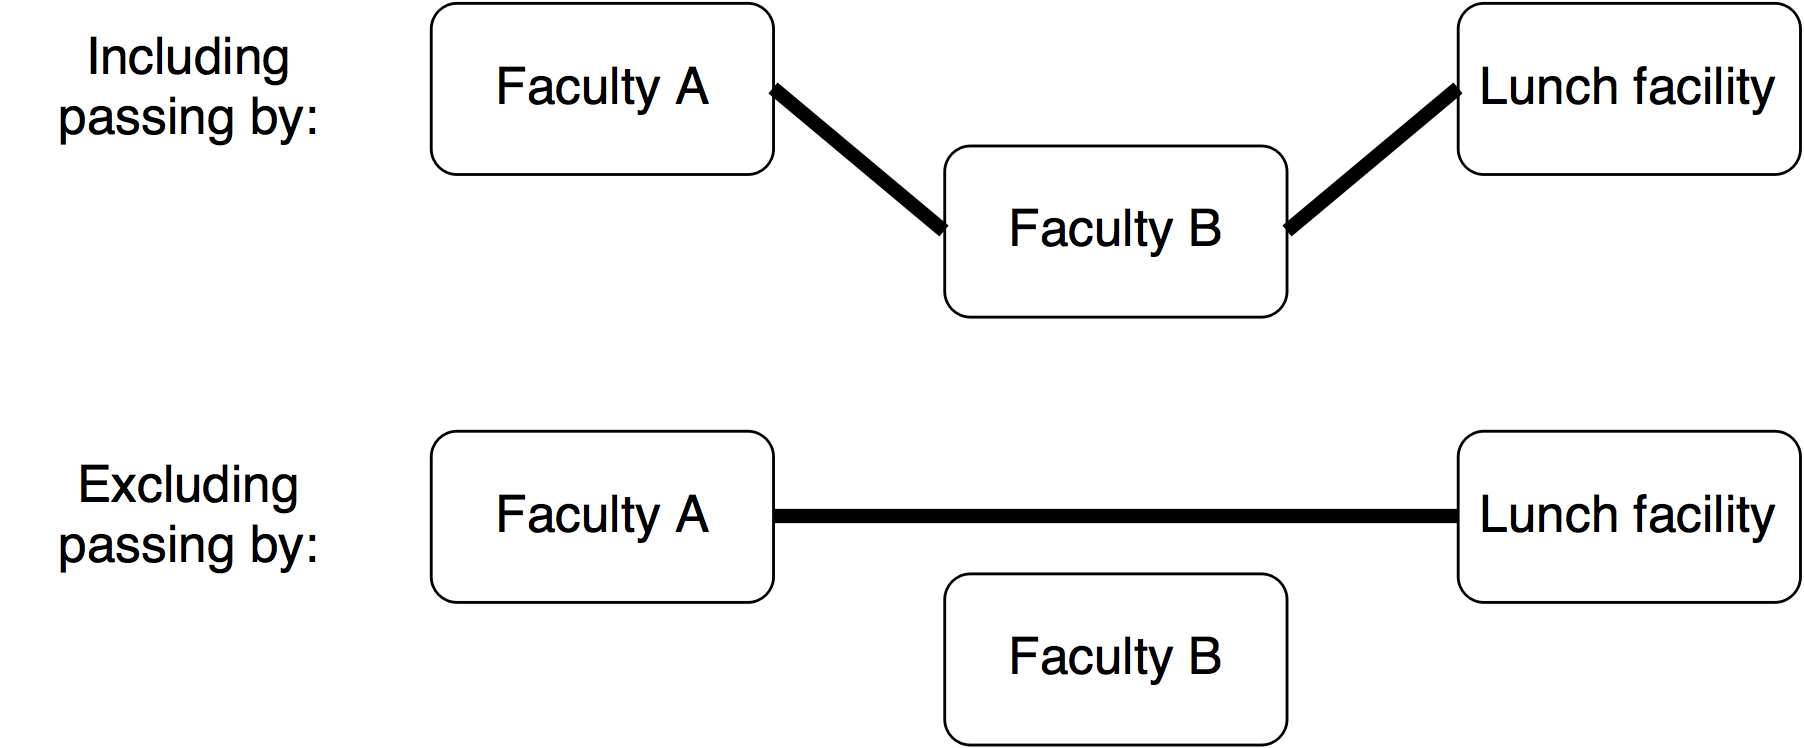
\includegraphics[scale=0.15]{PassingBy}
\captionsetup{justification=centering}
\caption{Passing by}
\label{figure:passing by}
\end{figure}
\subsection{Implementation}
The filling, grouping and filtering (passing by) steps described above are implemented in an integrated way. The Pseudocode for the implementation is shown in \autoref{kaas}. As can be seen in the code there is communication with the database at several points. The table from which the records are retrieved for each mac address is already processed as described in the general filtering section. Furthermore the format of the table is slightly different compared to the initial wifilog. The session duration is exchanged for an end time column which is derived by adding the session duration to the asstime (start time of a record).

\begin{figure}[H]
\centering
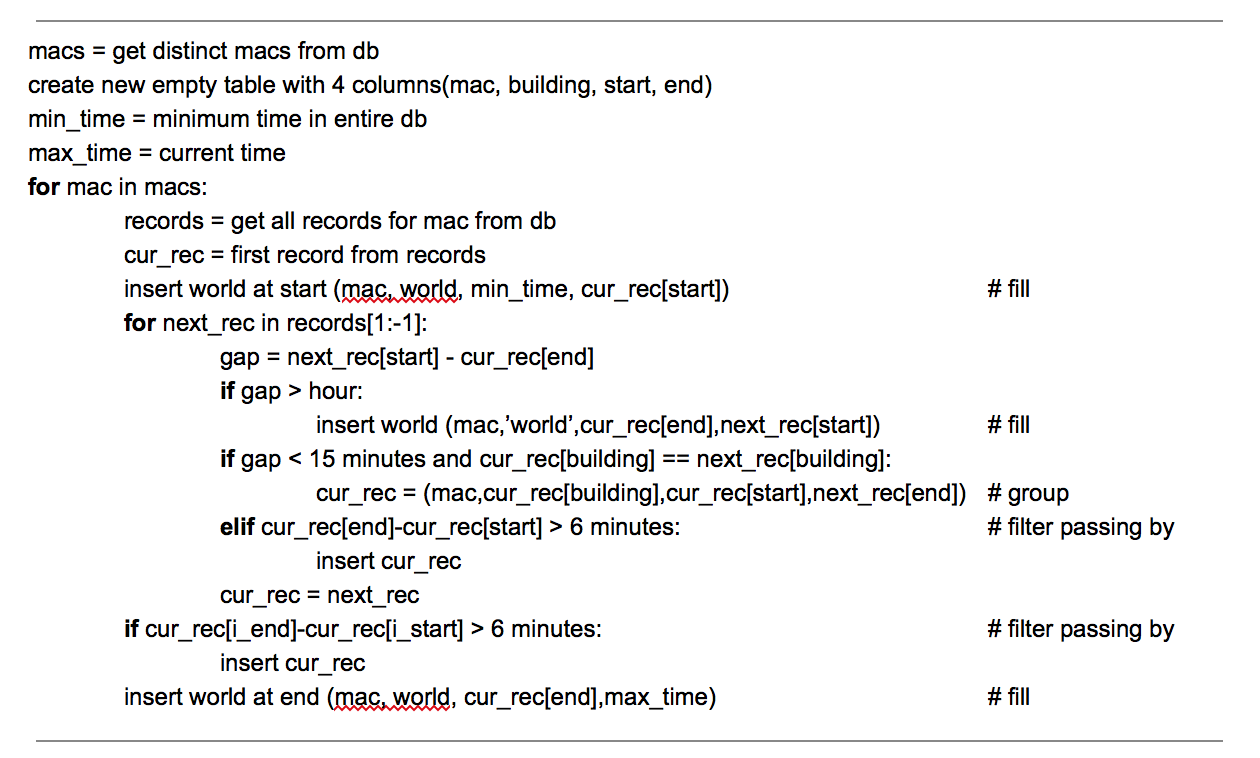
\includegraphics[scale=0.5]{pseudocode.png}
\captionsetup{justification=centering}
\caption{Pseudocode preprocessing}
\label{kaas}
\end{figure}

\autoref{preprocimg} shows an example of the records of one device over a time span of one day during the different pre-processing steps. From the raw data it can be seen that this person spends most of the day in building B. The person is scanned once at building A before he arrives in the morning and after what is likely to be his lunch break. The last two hours the person is scanned in building C. After filling three world records are added, at the beginning of the day, during the lunch break, and at the end of the day. The grouped records show that the subsequent scans in building B and C are grouped together. Finally the scans at building A are removed from the dataset as they are likely to indicate passing by events. 

\begin{figure}[H]
\centering
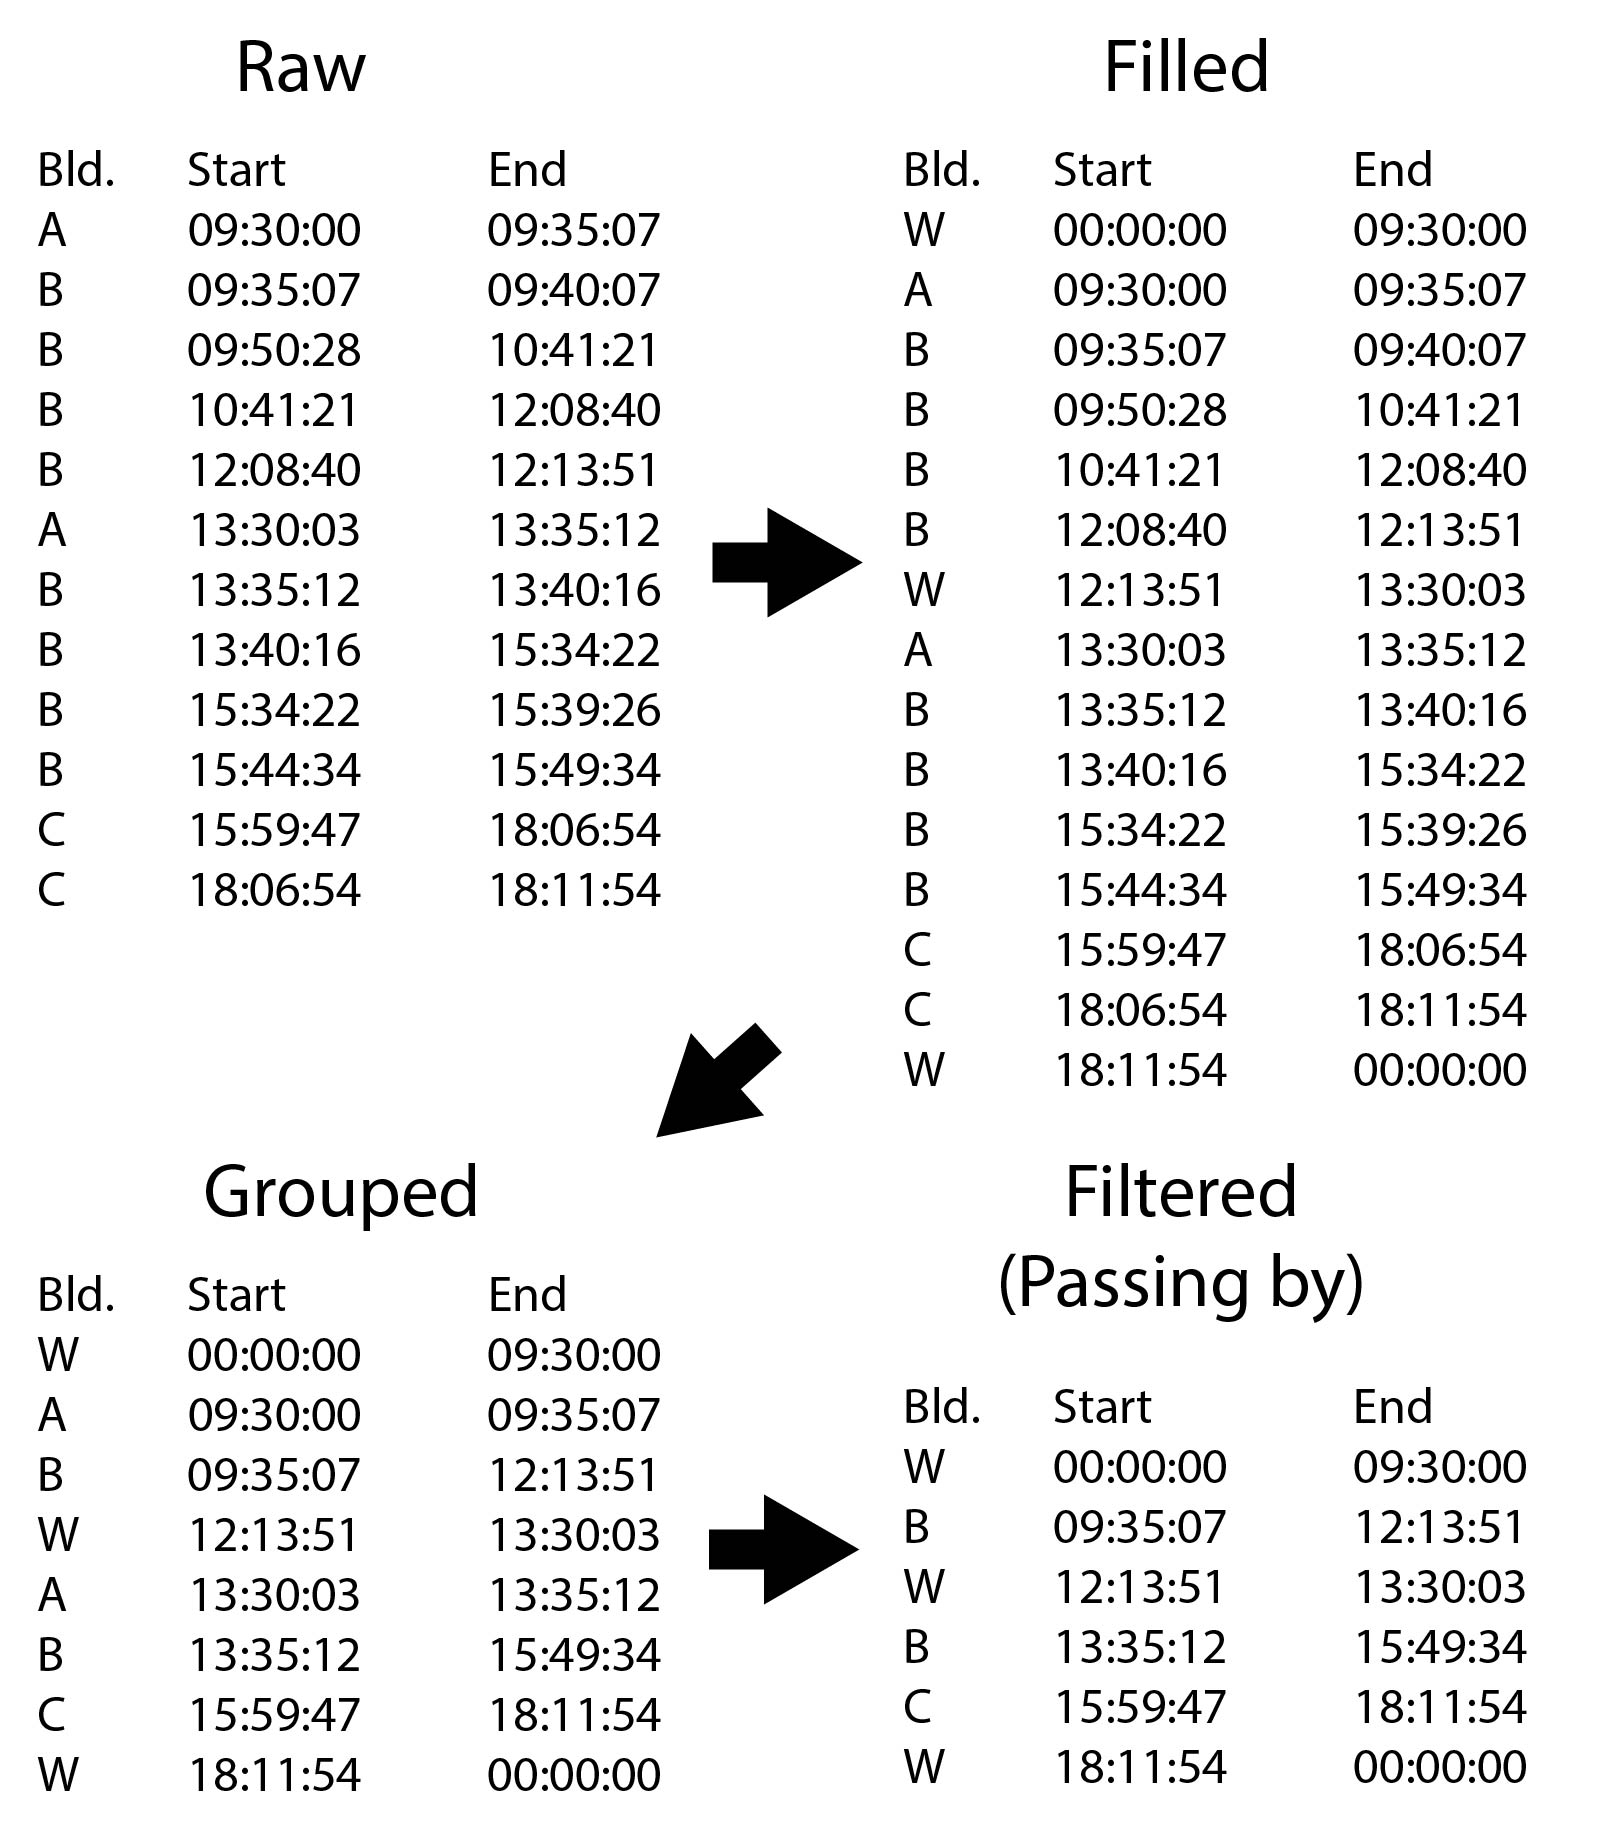
\includegraphics[scale=0.2]{PreProcessing-01.jpg}
\captionsetup{justification=centering}
\caption{Preprocessing}
\label{preprocimg}
\end{figure}


\subsection{Apname vs maploc}
The data in the table 'wifilog' contains information about the location of the Access Point (AP) in two columns. The first one is the column 'apname', which is a string with the symbolic name of the AP, for example 'A-08-G-010'. The two numbers in the second part of the string, in this case '08', represent the building number. This building number can be linked to a location in the world. 
The second column which contains information about location, is the column 'maploc'. This column also contains strings, which look as follows:

System Campus $>$ [buildingid] $>$ [specific location]'. An example of such a string is 'System Campus $>$ 21-BTUD $>$ 1e verdieping'. In such a string, the middle part can be linked to a building, so to a real-world location. 
But there are some other values for maploc, which can less clearly be linked to a real-world location. Such a value is 'Root Area', it is unclear what this value means and it contains no information about a building or area it might be in. This makes it impossible to link it to a location in the world. Then there is the value 'Unknown', a value that indicates that there was no name attached to the Access Point that user was connected to. Again in this case, it is impossible to link this value to a real-world location. 

As both 'Root Area' and 'Unknown' are in the minority of records, they could be left out of the queries. But for some records, the column 'apname' did provide information about the location, while the 'maploc' column value was 'Root Area'. In most of these cases however, the building number, the second part of the string, was a number of length three. But there are no buildings on the TU Delft campus with a building number that high. When consulting Wilko Quack about this, he explained that these building numbers had an arbitrary 1 in front of the building number. So 'A-134-A-001' was not building 134, but building 34, which was an actual building number on the campus. This would mean that using the column 'apname' for getting the building number would mean a higher number of results and therefore a more realistic visualization of the movements. 

Taking the substring of that column and linking it to a building with an actual location is done in two steps. First the whole string is retrieved and with a function in Python the substring is derived. Subsequently, the building id that is the result of this function can be linked to a table in the database which has for every building five columns: buildingid, name, point (as geometry), x (longitude), y (latitude) (see in \autoref{maps}).
\section{Movement between buildings}\label{movement between buildings}
To automate the workflow of creating movement visualizations between buildings, a program is created. There is a distinction between two types of visualization:
\begin{enumerate}
\item Maps
\item Bar charts
\end{enumerate}
The bar plot visualizes the movement throughout the day in 24 bars. Each bar represents the movement from a selection of buildings to another selection of buildings, over a time interval of one hour. In \autoref{barcharts}, the bar charts will be discussed in more detail. For map visualization the JavaScript Leaflet.js is used, this allows for creation of an interactive user interface with a base map from Open Street Maps and visualize the buildings and movement between them. In \autoref{maps} the map visualization will be discussed in more detail. For the bar charts the Python module matplotlib was used.
\subsection{Create movement records}

The data resulting from pre-processing contains the states of where a particular device was located during a certain time period. Implicitly this also includes information on the movement of the device. If a device is first located in building A and subsequently in building B it must have moved from building A to B. However, in order to be able to retrieve the movement patterns of devices the movement should be stored explicitly. This means that each record should store the movement of one device from one building to another building or to world. Examples of movement patterns that can be retrieved from this data are: the number of devices moving from building A to B within a given time period, and the peak in movement from building A to all other buildings. 
\\\\
To create records for each movement first the preprocessed data is ordered on mac address and start time. By doing this all the subsequent states for every device are listed directly below each other (see \autoref{figure:movementrecs}). As a movement is defined by the change of one state to another, movements records can be created from every two consecutive state records (see \autoref{figure:movementrecs}. However, not every two consecutive states represent a movement. Only when the two states concern the same device and they are at different buildings they represent a movement. This means that movement records with different mac addresses or similar building id’s are filtered out (see \autoref{figure:movementrecs}.\\
\\\\
\\\\
\\\\
\\\\
\\\\
\\\\
\\\\
\\\\

\begin{figure}[H]
\centering
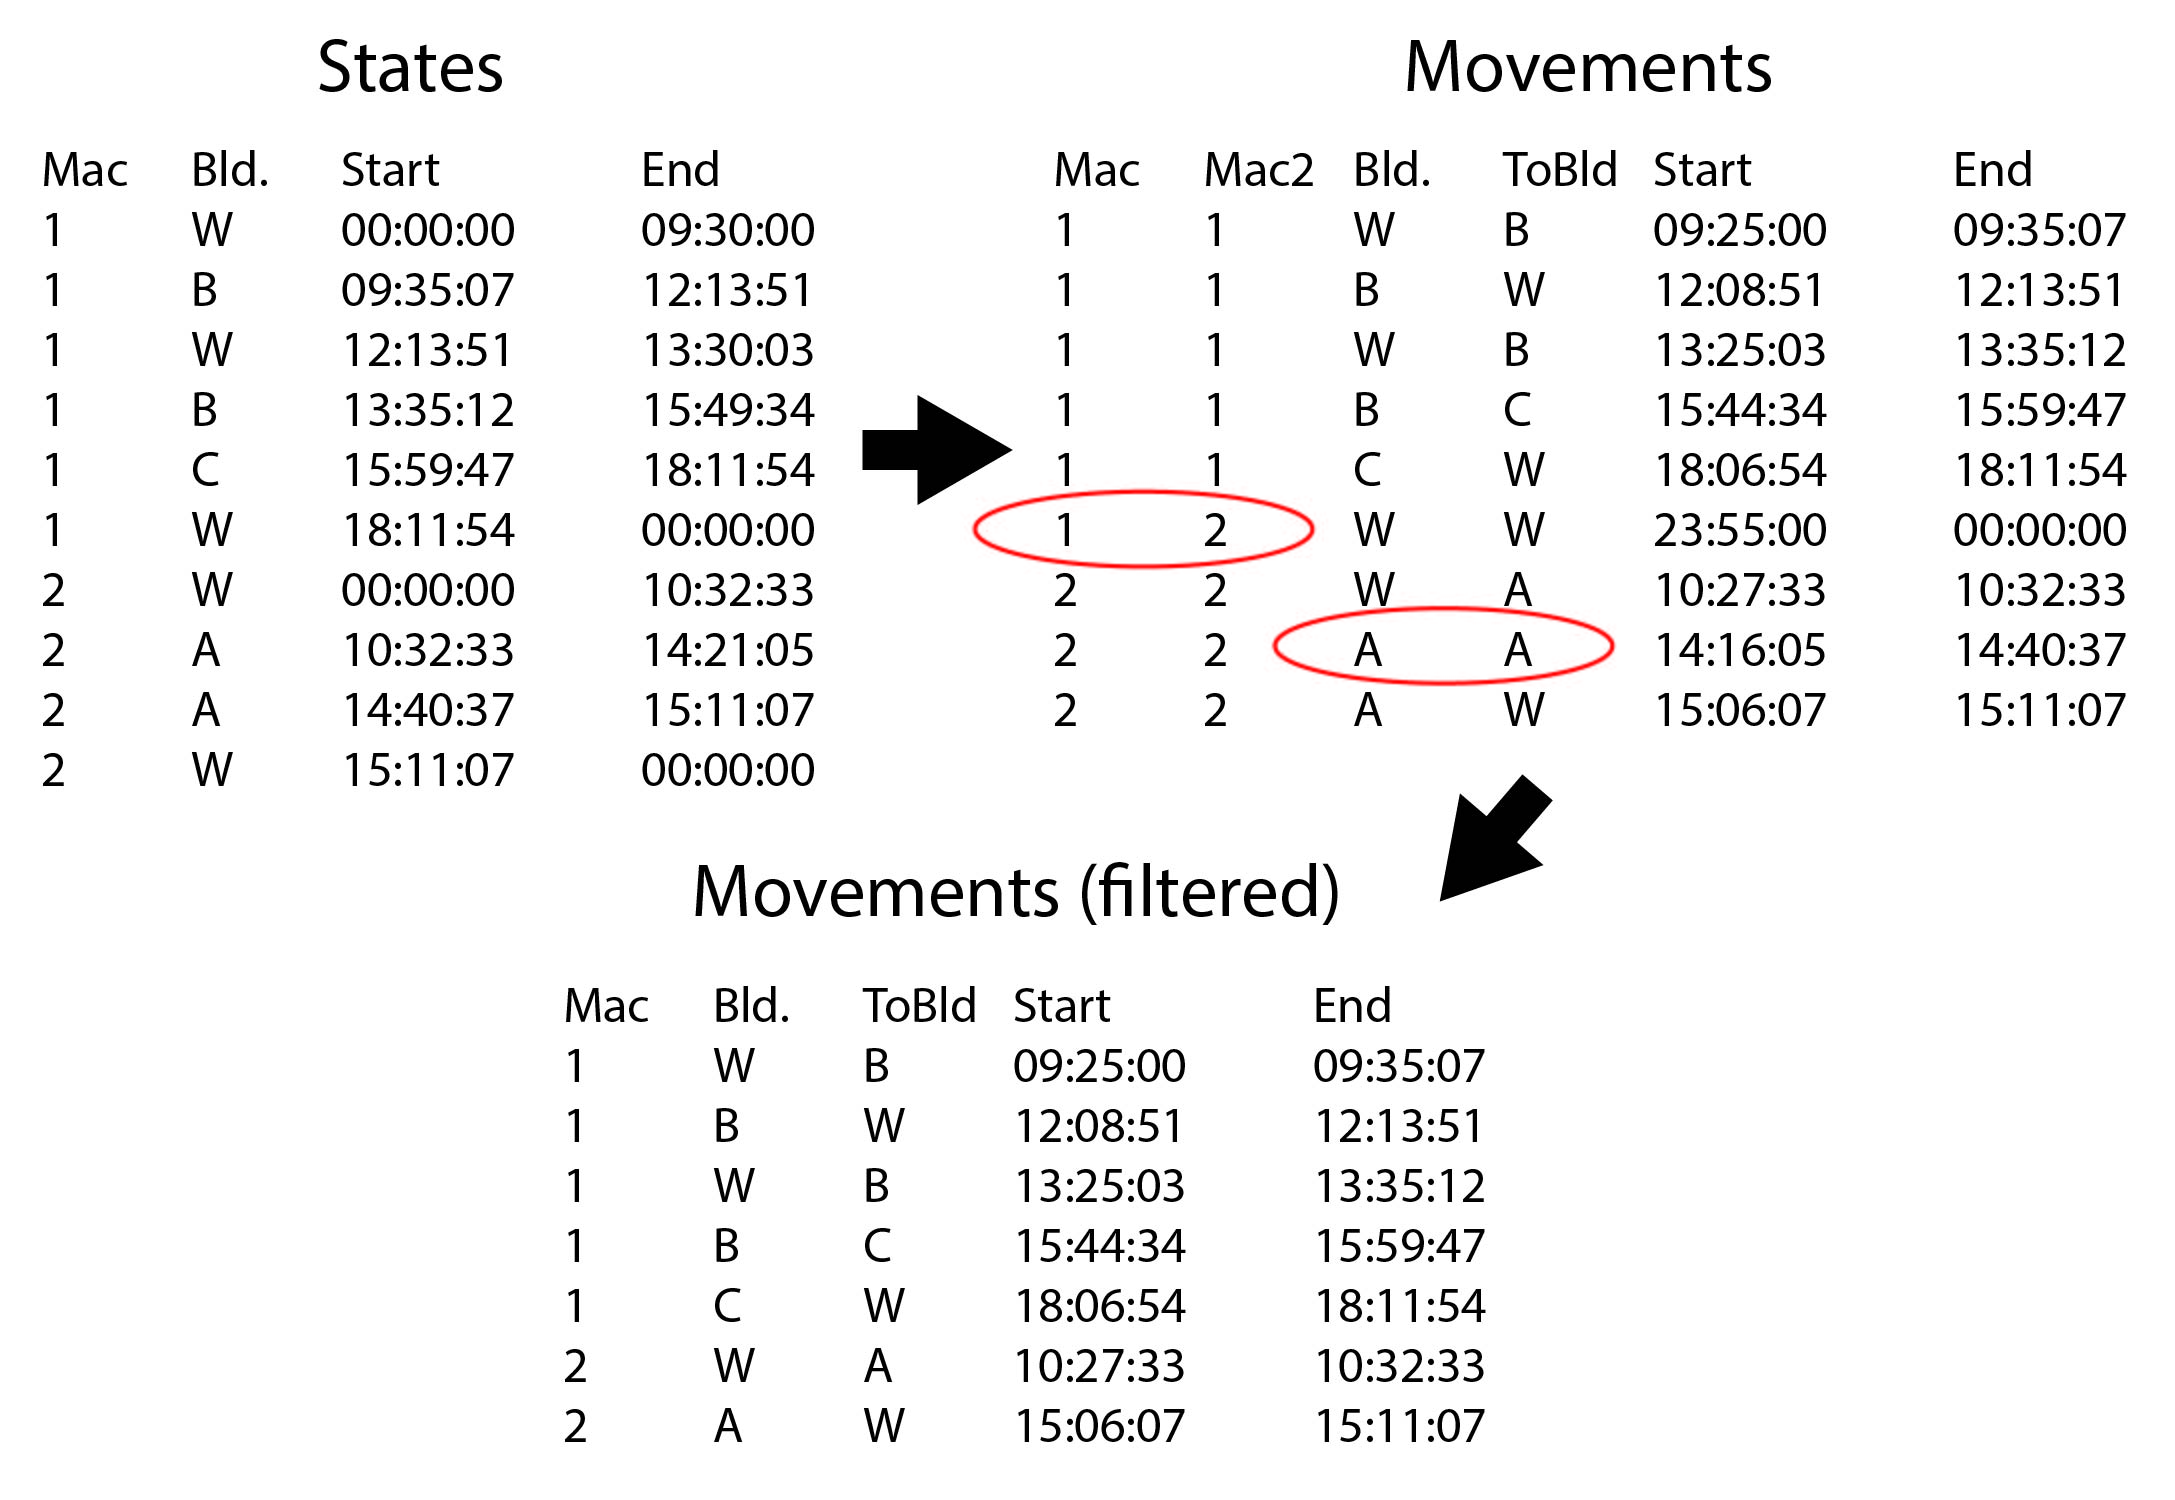
\includegraphics[scale=0.2]{movement_records.jpg}
\captionsetup{justification=centering}
\caption{Movement records}
\label{figure:movementrecs}
\end{figure}

The start and end time of the movement are defined by the end time of the previous state minus 5 minutes, and the start time of the next state (see \autoref{movement}). The reason that 5 minutes are subtracted from the end time of the previous state is that this is approximately the last moment in time the device was actually scanned at the location of the previous state. In the figure below the device is scanned 15:21 at building B. Approximately 5 minutes later (at 20:27) the device is scanned at building C. The state record of building B however continues all the way until 20:27, whilst the last time it was actually scanned at building B was 15:21. As a result it can be concluded that the movement from building B to C took place somewhere between 15:21 and 20:27. Therefore the start time of the movement between B and C can be approximated by subtracting 5 minutes from the end time of the state record at B. As can be observed in the movement from A to B is retrieved in the same way.

\begin{figure}[H]
\centering
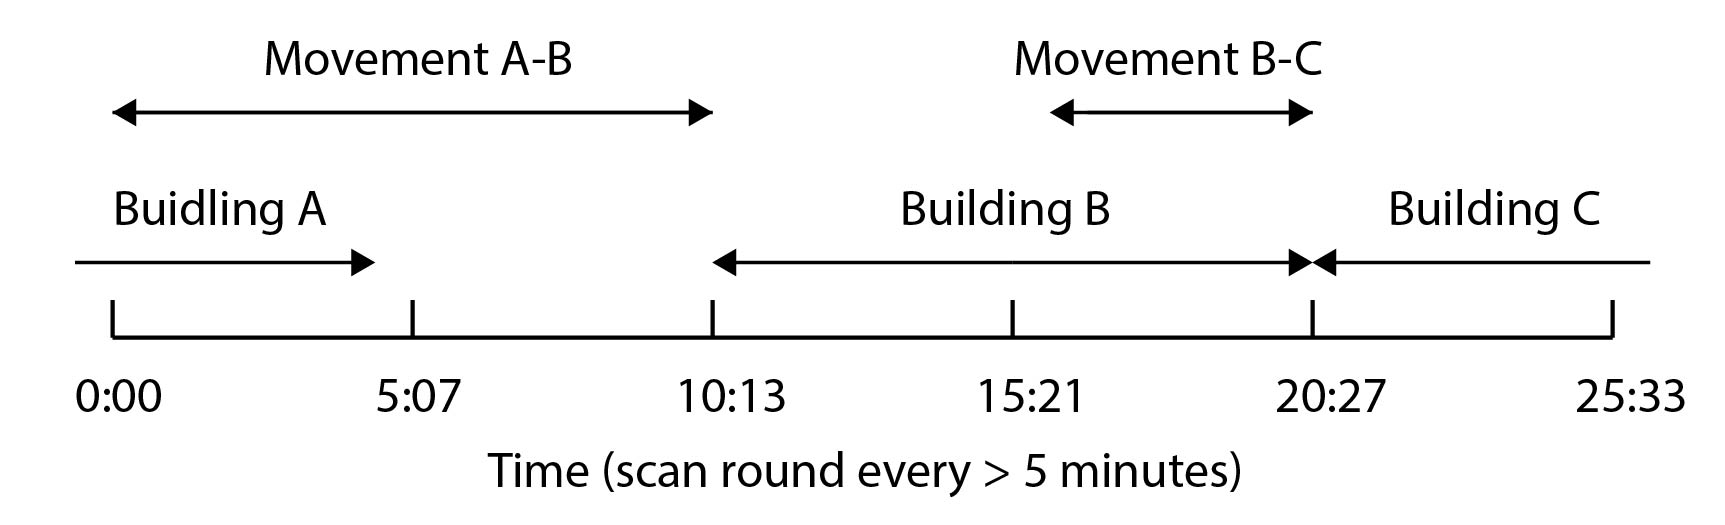
\includegraphics[scale=0.2]{movement.jpg}
\captionsetup{justification=centering}
\caption{Movement}
\label{figure:movement}
\end{figure}


\subsection{Movement over time}

As the described in section \autoref{GUI} the GUI allows a user to select particular days and specify origin and destination buildings of the movement. Based on this input the movement table can be filtered. Finally the filtered data can be visualized as the amount of movement between the specified buildings at each hour of the day. If the user has specified multiple days, the average amount of movement of these days is taken. It should be noted that the amount of movement is defined by the number of devices moving between the specified buildings. \autoref{figure:weekdays_2} gives an example of the visualization of movement over time.
\begin{figure}[H]
\centering
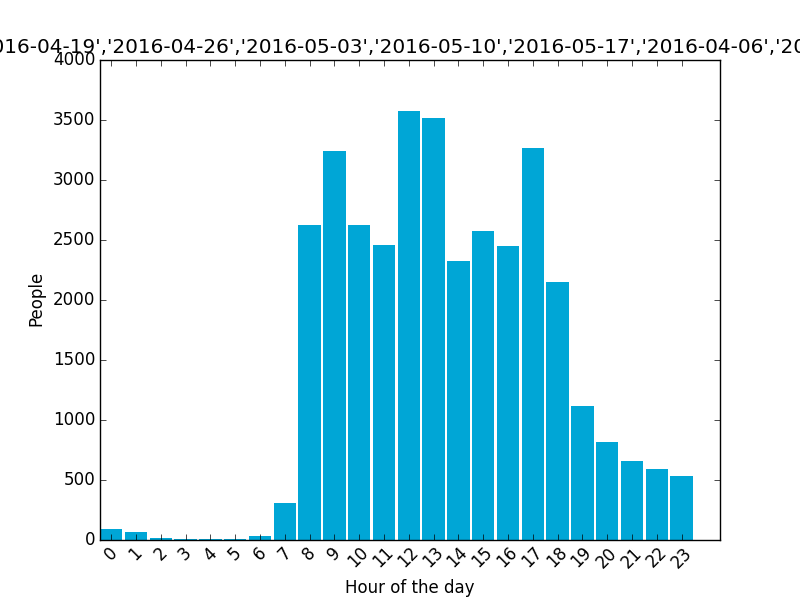
\includegraphics[scale=0.5]{12_weekdays.png}
\captionsetup{justification=centering}
\caption{Movement overtime}
\label{figure:weekdays_2}
\end{figure}


\subsection{Graphical User Interface}\label{GUI}
The Graphical User Interface (hereinafter referred to as GUI) for this work is a Python program that shows a Tkinter interface. When the user runs the program, it will display a main window, which is shown in \autoref{figure:GUImain}
\begin{figure}[H]
\centering
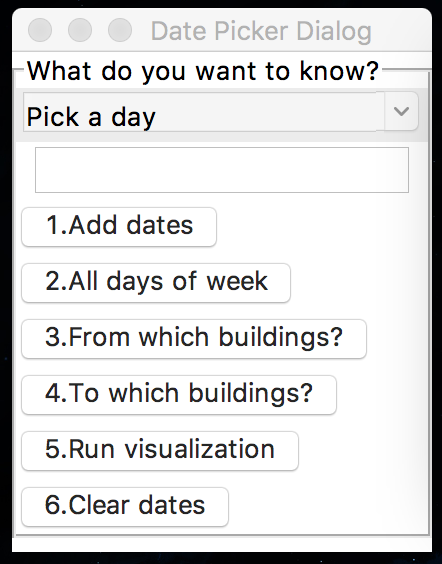
\includegraphics[scale=0.7]{GUI-main}
\captionsetup{justification=centering}
\caption{main window of GUI}
\label{figure:GUImain}
\end{figure}
\pagebreak 
To create a visualization, the user first has to select a time interval and then the buildings from and to which the movement should be visualized. The user has 2 options to select the time series for the current visualization:
\begin{enumerate}
\item Click on '1. Add dates' which will open the date picker dialog
\item Pick a day from the dropdown menu and click on '2. All days of week' 
\end{enumerate}

\begin{figure}[H]
\centering
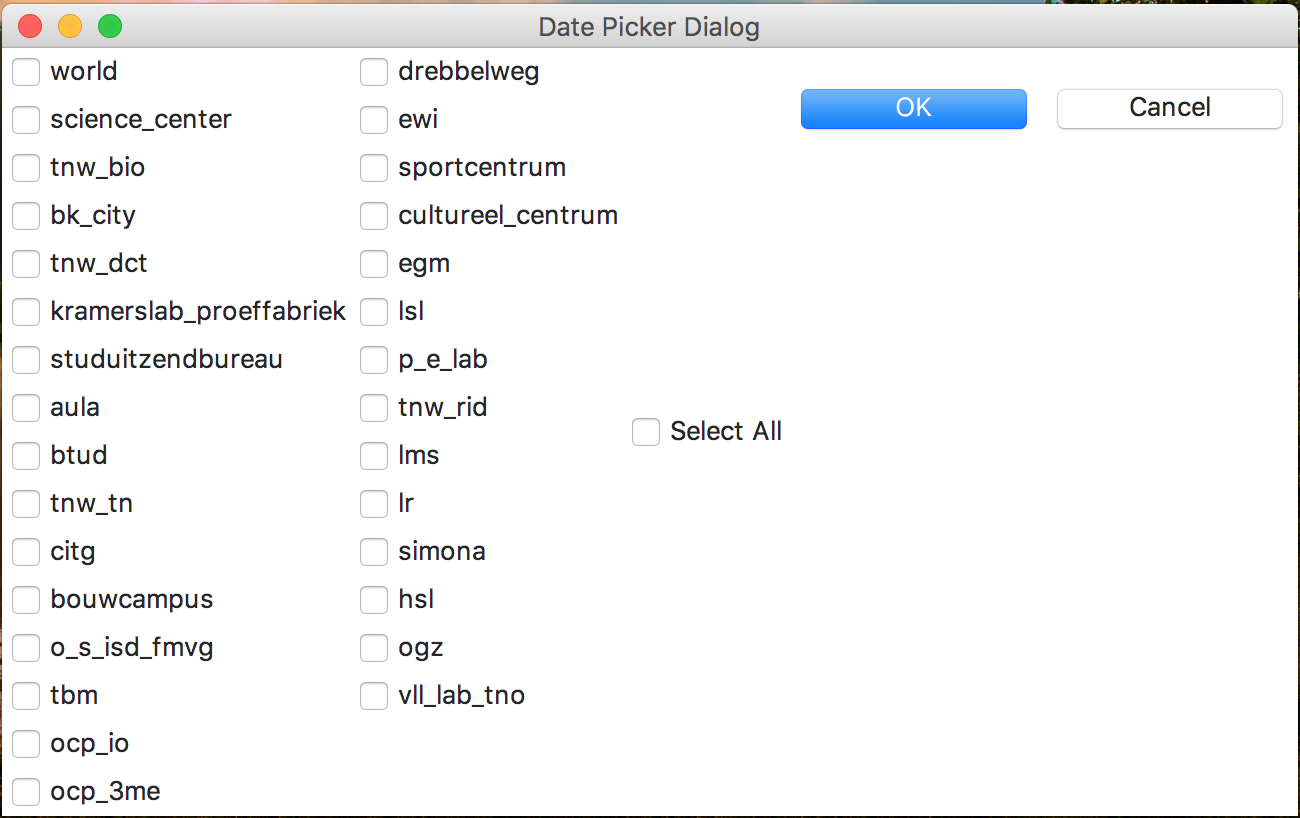
\includegraphics[scale=0.5]{GUI-buildings}
\captionsetup{justification=centering}
\caption{Buildings selection}
\label{figure:GUIbuildings}
\end{figure}

\begin{figure}[H]
\centering
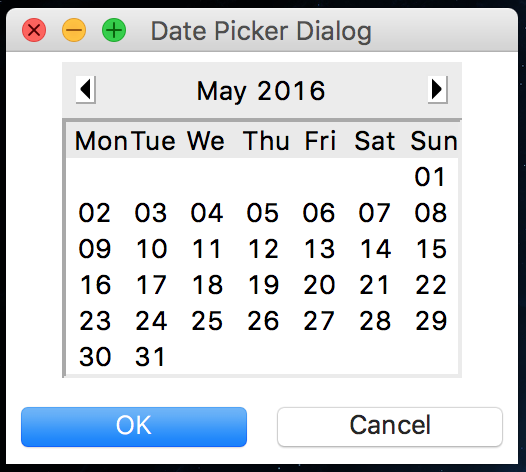
\includegraphics[scale=0.7]{GUI-dates}
\captionsetup{justification=centering}
\caption{Dates selection}
\label{figure:GUIdates}
\end{figure}

Option 1 can be used to select particular days without order. Option 2 can select 'every Tuesday' or even multiple recurring dates, such as 'every Monday to Friday'. It is also possible to combine option 1 and 2 to have for example 'every Monday and Friday the 13th of May'. 

After selecting the time series, the user has to select the buildings from and to which the movement should be visualized. The 3rd and 4th button bring up the same dialog. This dialog shows checkboxes for every building. Every building that is check will be visualized. The user also has the option to select all buildings. If the user would like to see movement from and to the same building, the user can select the same buildings twice.

\subsection{Maps}\label{maps}
In order to get an overview about how people move on the campus and further more,  find out movement patterns, a map visualization is essential. Map visualization consists of three parts: 
\begin{enumerate}
\item base map: open street map is used as a base map. There are many labels on open street map, providing more context of the environment, so it is more clear and readable compared to other base maps like satellite images.
\item building markers: building markers show the locations of the buildings. Google maps marker style is used since it is commonly used in many map application. Because the shape of the building is not useful in analyzing movement patterns between buildings, each building is regarded as a point instead of a polygon, thus a node in the network, 
\item lines: lines are the most essential part in map visualization, they represent movements between buildings.
\end{enumerate}

In the first stage of map visualization, only base map and lines are taken into consideration, building markers are not shown on the map. The line width represents the amount of movement and movements are aggregated daily regardless of the timestamp of each movement during a day. This map visualization gives an overview of the movements over a day and between which buildings there are the most movements. The following maps show the difference of the amount of movement between April 11th (weekday) and April 17th (weekend).

\begin{figure}[H]
\captionsetup[subfigure]{justification=centering}
    \centering
    \begin{subfigure}[t]{0.5\textwidth}
        \centering
        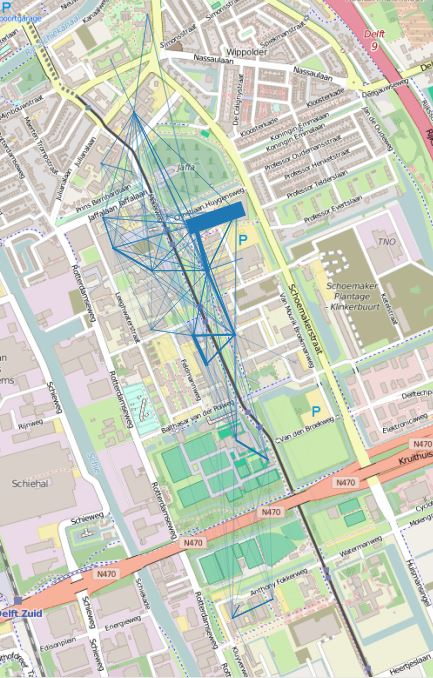
\includegraphics[scale=0.85]{pic1}
        \caption{April 11th, weekday}
    \end{subfigure}%
    ~ 
    \begin{subfigure}[t]{0.5\textwidth}
        \centering
        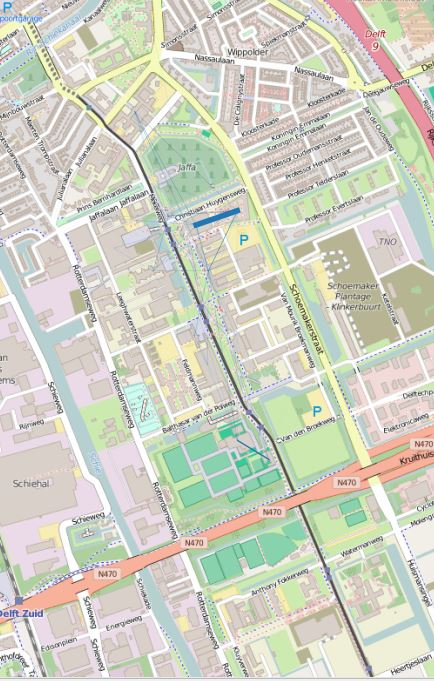
\includegraphics[scale=0.85]{pic2}
        \caption{April 17th, weekend}
    \end{subfigure}
    \captionsetup{justification=centering}
    \caption{Static visualization}
    \label{staticvisualization}
\end{figure}

It's clear that between Aula and library, there are the most movements and the amount of movements is totally different on weekday and on weekend.

Given that movements are dynamic and occuring in both space and time, a dynamic map visualization is created to display individual movement over a day with temporal information. The following screenshots of the gif file show how the movements look like at a certain time of a day:

\begin{figure}[H]
\captionsetup[subfigure]{justification=centering}
    \centering
    \begin{subfigure}[t]{0.3\textwidth}
        \centering
        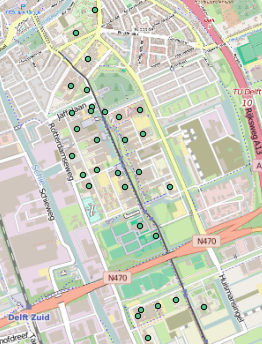
\includegraphics[scale=0.6]{frame009}
        \caption{7:00 am}
    \end{subfigure}%
    ~ 
    \begin{subfigure}[t]{0.3\textwidth}
        \centering
        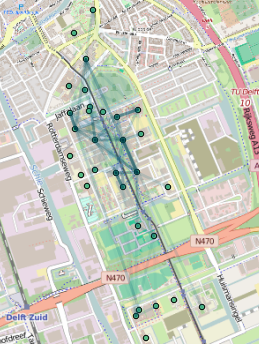
\includegraphics[scale=0.6]{frame021}
        \caption{9:00 am}
    \end{subfigure}
    \begin{subfigure}[t]{0.3\textwidth}
        \centering
        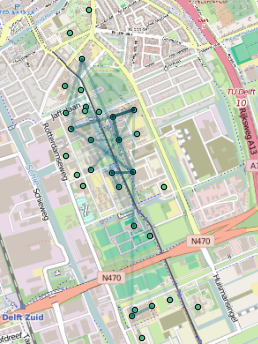
\includegraphics[scale=0.6]{frame033}
        \caption{11:00 am}
    \end{subfigure}
    \begin{subfigure}[t]{0.3\textwidth}
        \centering
        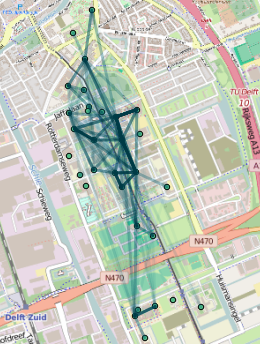
\includegraphics[scale=0.6]{frame045}
        \caption{13:00 pm}
    \end{subfigure}
    \begin{subfigure}[t]{0.3\textwidth}
        \centering
        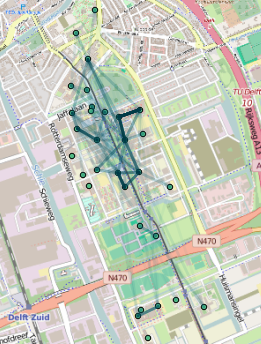
\includegraphics[scale=0.6]{frame057}
        \caption{15:00 pm}
    \end{subfigure}
    \begin{subfigure}[t]{0.3\textwidth}
        \centering
        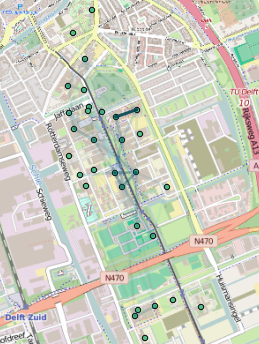
\includegraphics[scale=0.6]{frame066}
        \caption{16:30 pm}
    \end{subfigure}
    \begin{subfigure}[t]{0.3\textwidth}
        \centering
        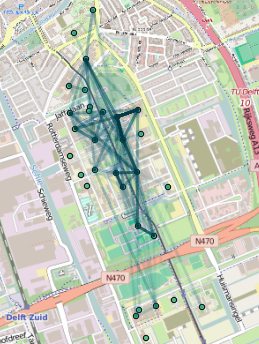
\includegraphics[scale=0.6]{frame075}
        \caption{18:00 pm}
    \end{subfigure}
    \begin{subfigure}[t]{0.3\textwidth}
        \centering
        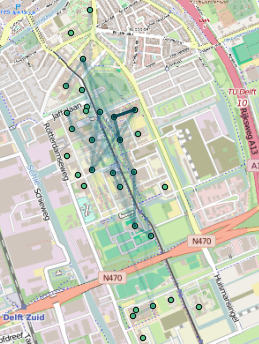
\includegraphics[scale=0.6]{frame087}
        \caption{20:00 pm}
    \end{subfigure}
    \begin{subfigure}[t]{0.3\textwidth}
        \centering
        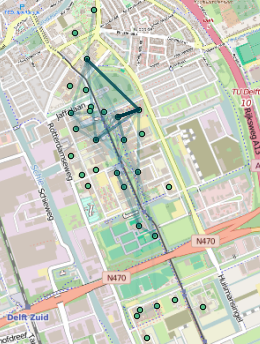
\includegraphics[scale=0.6]{frame099}
        \caption{22:00 pm}
    \end{subfigure}

    \captionsetup{justification=centering}
    \caption{Dynamic visualization of movements, April 11th}
    \label{autovisualization}
\end{figure}

In these pictures, the more movements there are, the less transparent the lines are. So generally speaking, from 7:00 am to 20:00 pm, there are two peaks at 13:00 pm and 18:00 pm. Hence, it is possible to get some insights about movement patterns from the animation. However, the dynamic map visualization doesn't provide detailed information to dig into but only an overview. So in order to find movement patterns, it is necessary to create maps containing more information, including time, direction and so forth. 

Because the amount of data is big, it is more convenient to generate maps automatically so that it will fasten the progress of finding movement patterns. According to the three components of map, there is some information needed to be collected before visualizing movement on map. The locations of buildings are collected manually on Google earth based the campus map. These locations are exported as KML file and imported into QGIS. After adding geometry columns x and y, the csv file is created and imported into database. By using $ST\_MakePoint$ function, a geometry column is created in database. In summary, the building locations are stored as the structure described in following table:

\begin{table}[H]
\centering
\begin{tabular}{|c|c|c|c|c|}
\hline 
id & name & geometry & x & y \\
\hline
0 & world & & & \\
\hline
3 & science\_ center & 010100000042A7.. & 4.36939919846287 & 52.0072322181367 \\
\hline
5 & tnw\_ bio & 010100000043AE.. & 4.37120211221402 & 52.0086132164098 \\
\hline
8 & bk\_ city & 010100000077E3.. & 4.37053698152436 & 52.0056562098059 \\
\hline
12 & tnw\_ dct & 01010000007CA.. & 4.36891378927259 & 52.0040834950037\\
\hline
.. & ... & ....& .... &....\\
\hline	
\end{tabular}
\captionsetup{justification=centering}
\caption{Building data structure}
\label{table:building}
\end{table}

There is a special 'building' called $world$ in the database. It is not an actual location, it is a virtual location which is used if someone is not scanned on the campus in a period of time. After storing the locations of buildings in the database, these locations will be extracted automatically from database to generate maps. There are two properties of lines used to deliver information:
\begin{enumerate}
\item width: line width is used to represent the amount of movements, but the amount is aggregated for both directions.
\item color: color is gradient from red to green. Red line means the movement is not symmetric that much more people move in one direction than the other, while green line means the movement is symmetric.
\end{enumerate}

Based on this map visualization, users can choose certain dates and certain buildings to generate maps automatically. It makes it easier to find out movement patterns. Since not all buildings are chosen, the map will only display the movements between several buildings, which makes the map more readable:
\\\\
\\\\
\\\\
\\\\
\\\\
\\\\

\begin{figure}[H]
	\centering
	\captionsetup[subfigure]{justification=centering}
	\begin{subfigure}[t]{0.48\textwidth}
	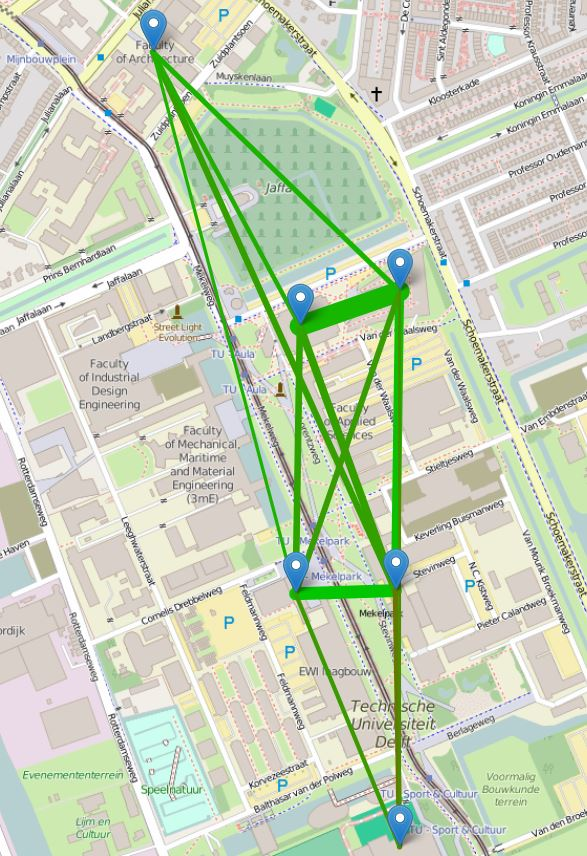
\includegraphics[scale=0.6]{pic3}
	\caption{Amount of movements on April 25th}
	\end{subfigure}
	\begin{subfigure}[t]{0.48\textwidth}
	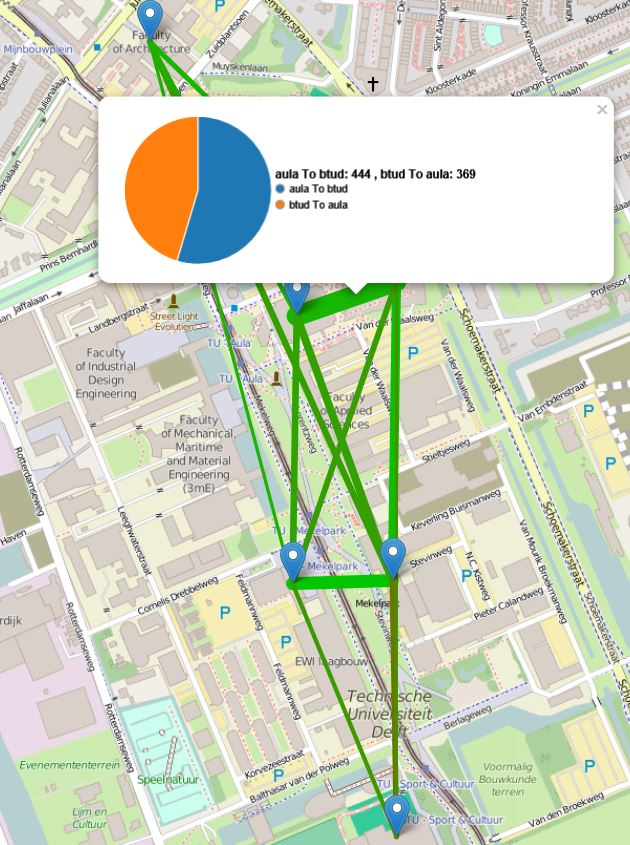
\includegraphics[scale=0.6]{pic4}
	\caption{Amount of movements in pie chart}
	\end{subfigure}
\end{figure}

As shown in the map, the lines are in different colors, which shows the symmetry of the movements. If the user is willing to know more about the movement, it is also possible to click on the line to check the amount of the movements for each direction in detail, and there will be a pie chart showing how symmetric the movements are. With the map visualization, it is easy to focus on movements which are special or interesting.

\section{Trajectories}\label{trajectories}
This GSP attempts to identify people’s movement patterns from anonymized wifilogs. To solve this problem, individual trajectories must be discovered. The data provided by the eduroam network enables a detailed view of people’s movement on campus. The large coverage of the eduroam network allows to track users for a large part of the day when they enter the campus. However, the obeservation space is limited to the extent of the size of the campus, making it not possible to track people outside the eduroam network. A second disadvantage is the spatial resolution of the positioining method. The size of each Wi-Fi cell determines the spatial resolution, as the location of mobile devices is estimated at the origin of a AP. The size of each Wi-Fi cell depends on the distribution of APs. For indoor environments of the TU Delft campus, this is just a few tens of meters wide. This resolution allows tracking movement at a building level by re-locating mobile devices to the closest AP. Data between two re-locations is not available. Therefore, an individual’s trajectory is depicted by connecting the re-locations as a sequence of APs. These individual trajectories are used to identify patterns. 

First, this chapter will describe the extraction of locations of a user. Then the mining of individual trajectories from a anonymized Wi-Fi scanlist is described. Subsequently, the mining of movement patterns in time or space is described. 

\subsection{Location extraction}
A location represents a geographic position where a user stays. For identifying movement patterns from Wi-Fi monitoring, we are interested in movement between two locations where an individual stays for a longer time period. Such a location, or stay place, can be detected when a user is connected to the same AP for a longer time. To detect  buildings as a location (i.e. contains multiple APs), two consecutive WiFi scans must contain  APs of the same building. With a data collecting interval of 5 minutes, it means that people will be filtered out if their stay duration is less than 10 minutes. Based on this assumption, people with a shorter stay duration are considered passing by.

\subsection{Individual trajectory}
An individual’s trajectory is constructed as a sequence of locations in order of the scan time. Start and end time of a trajectory can be specified with a time interval, e.g. a day or week. If p is a location, then a trajectory can be written as:
$$p1 \rightarrow p2 \rightarrow p3 \rightarrow …\rightarrow pn$$

Given a time interval, there is a set of individual trajectories S = \{t1, t2, t3,...,tn\} where each ti is the trajectory over a time interval of one user. 

\subsection{Trajectory Pattern}
From a set S of trajectories, different patterns can be identified using seqeuntial pattern mining algorithms. Frequency of a trajectory by all users of the campus can be detected. This can be represented as a trajactoy T with a support s. Support means how many times the same sequence, or sub-sequence, is shared in the set of trajectories. This gives valuable information on the order common buildings are used and what order of buildings occurs the most. Furthermore, the lenght of a trajectory can be discovered. This allows for identification of movement patterns of a specific lenght n. Also, when location is not considered, but only the lenght of a trajectory, the mobility pattern of an individual can be discribed in terms of how many times he/she re-locates. 

\section{Associated buildings}\label{Associated buildings}

The following section describes how movement patterns were derived on building level, without considering the direction or order of the movement. An association rule mining algorithm \parencite{agrawal_mining_1993} was used to identify groups of buildings that frequently visited in combination with each other. Firstly the algorithm is described briefly, then the results are presented.
\subsection{Association rules mining}
Association rule mining is a technique to analyse what variables or items are commonly associated with each other in large databases. Probably the one of the main application is to analyse which items are commonly bought together by customers of a supermarket. As an example for this use case is an association rule of an itemset \{bread, butter\}, tells that in 80\% of those transactions including \{bread, butter\}, also \{milk\}  was present. In other words, 80\% of the people who buy bread and butter also buy milk \parencite{agrawal_mining_1993}. Compared to sequence mining, association rule mining does not consider the order of items neither within, nor across transactions.

Thus every rule is composed by two itemsets, the \textit{antecedent} \{bread,butter\} on the left-hand side, and the \textit{consequent} \{milk\} on the right-hand side. The rule is denoted as \{bread, butter\} \verb|=>| \{milk\}.

\subsection{Assosication rules of buildings}
When a trajectory is simplified into a set of distinct buildings that the person
visited, association rules for buildings can be derived. In this case the rule
describes the set of buildings, or buildingset, that are commonly visited in
combination. For example the rule \{BK\_City, Aula\} \verb|=>| \{Library\}
tells that a group of people who visited the buildings BK\_City and Aula also
visited the Library.

As association rule mining does not consider the order of buildings, nor the
time spent in a building, it is important that these variables are appropriately
handled and noise is filtered out prior running the algorithm.

In the first version the buildingsets were stored in a table as below, where the
field \textit{mac} contains the mac-address of a device and each remaining field
represents a building. Value 1 is given if the device was recorded in a
building, otherwise no value is given. This binary encoding is rather simplistic
as it does not consider the amount of time spent in a building and therefore it
does not allow to differentiate between occasional or regular visits.

\begin{table}[H]
\centering
\captionsetup{justification=centering}
\caption{uncategorized buildingset table}
\label{uncategorized buildingset table}
\begin{tabular}{lllllll}
\cline{1-7}
mac & aula & bk\_city & bouwcampus & btud & ctig & ... \\ \cline{1-7}
A   & 1	& 1    	&        	&  	& 1	& 	\\
B   &  	&      	& 1      	& 1	&  	& 	\\
C   &  	& 1    	&        	&  	& 1	& 	\\
D   & 1	&      	&        	&  	&  	& 	\\
E   & 1	&      	& 1      	&  	&  	& 	\\ \cline{1-7}
\end{tabular}
\end{table}

Therefore in the second version a distinction between \textit{occasional,
regular} and \textit{frequent} stays was added to the buildingsets. The division
between the categories is based on the 40 hour workweek and 1.5 hour lecture
durations (see \autoref{table:stay duration categories}). 

\begin{table}[H]
\centering
\captionsetup{justification=centering}
\caption{Stay duration categories}
\label{table:stay duration categories}
\begin{tabular}{lll}
\cline{1-3}
Category   & hours/week           	& ID \\ \cline{1-3}
occasional & $\leq 0.5$             	& 1  \\
regular	& $\textgreater 0.5, \leq 5$ & 2  \\
frequent   & $\textgreater 5$       	& 3
\end{tabular}
\end{table}

The trajectories of approximately 14,000 devices were used to create the first set of association rules with categorized stay duration. At this stage only the noise was filtered from the data but not the stationary devices, and people carrying two devices were not accounted for. The time range of trajectories spanned from 31.03.2016 to 02.05.2016, approximately one month.

Although there are several measures to evaluate the interestingness of an association rule \parencite{zhang_survey_2009}, only \textit{support} and \textit{confidence} were used for testing purposes. 

\textbf{Support}
“The support for a rule is defined to be the fraction of transaction in the dataset that satisfy the union of items in the consequent and antecedent of the rule.” \parencite{agrawal_mining_1993}. In case of the rule \{BK\_City, Aula\} \verb|=>| \{Library\}, the support is the percentage of the total dataset that includes BK\_City, Aula and Library.

\textbf{Confidence}
Confidence measures the strength of the rule, and is considered as a conditional probability. In case of the rule \{BK\_ City, Aula\} \verb|=>| \{Library\}, the confidence is the probability that Library is in the trajectory if both BK\_ City and Aula are in the trajectory (\cite{agrawal_mining_1993}; \cite{anbukkarasy_interesting_2013}).

The most interesting rules are displayed in \autoref{figure:buildingset}:
\begin{figure}[H]
\centering
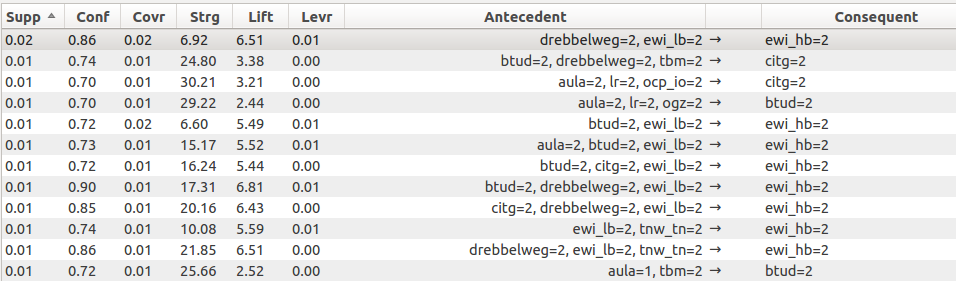
\includegraphics[scale=0.45]{acc_buildingset_v0516}
\captionsetup{justification=centering}
\caption{Building set}
\label{figure:buildingset}
\end{figure}

In the buildingset of approx. 14,000 devices 2\% was recorded in all of the buildings \textit{Drebbelweg, EWI-LB, EWI-HB} (Support = 0.02). There is an 86\% chance that if a device is recorded in the buildings \textit{Drebbelweg, EWI-LB}, then it is also recorded in \textit{EWI-HB} (Confidence = 0.86). And they spent on average between half hour to five hours a week in each building (drebbelweg=2, ewi\_ lb=2, ewi\_ hb=2).

\section{Entrances and exits}\label{entrances and exists}
This section will describe the undergoing process in order to know how frequent the entrances and exits of a building are used. Knowing this will give insight into the use of a building, the spatial context and the relation between these two. Our hypothesis is that access points located near the entrance(s) of a building are most frequently used as first access point when entering a building, and as last access point when leaving a building. Firstly, an approach will be presented that does not take in account that devices might get scanned when passing by the building. In the second approach we will make use of the pre-processed data which excludes the devices that get scanned when passing by the building. 

\subsection{First approach:including devices passing by}
The first approach makes use of the raw wifilog data, by finding the part in a sequence in which a device is scanned by an access point in a building and is subsequently scanned in another building. With the location of the access points known, we hope to get insight into the use of an entrance or exit location in a building. 
\begin{figure}[H]
\centering
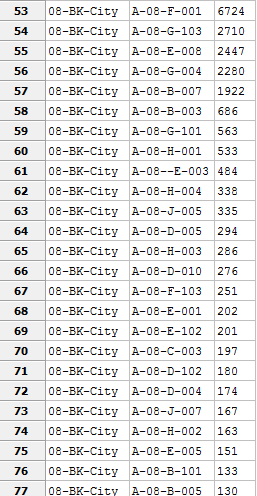
\includegraphics[scale=0.45]{entrances_firstapproach_bk}
\captionsetup{justification=centering}
\caption{A segment of the resulting table after querying}
\label{figure:Entrance1ApproachTable}
\end{figure}

The stays in which the device is scanned once are not filtered out. These single scans imply that a person with the device only passed by the building, thus was not really located in the building. 

\begin{figure}[H]
\centering
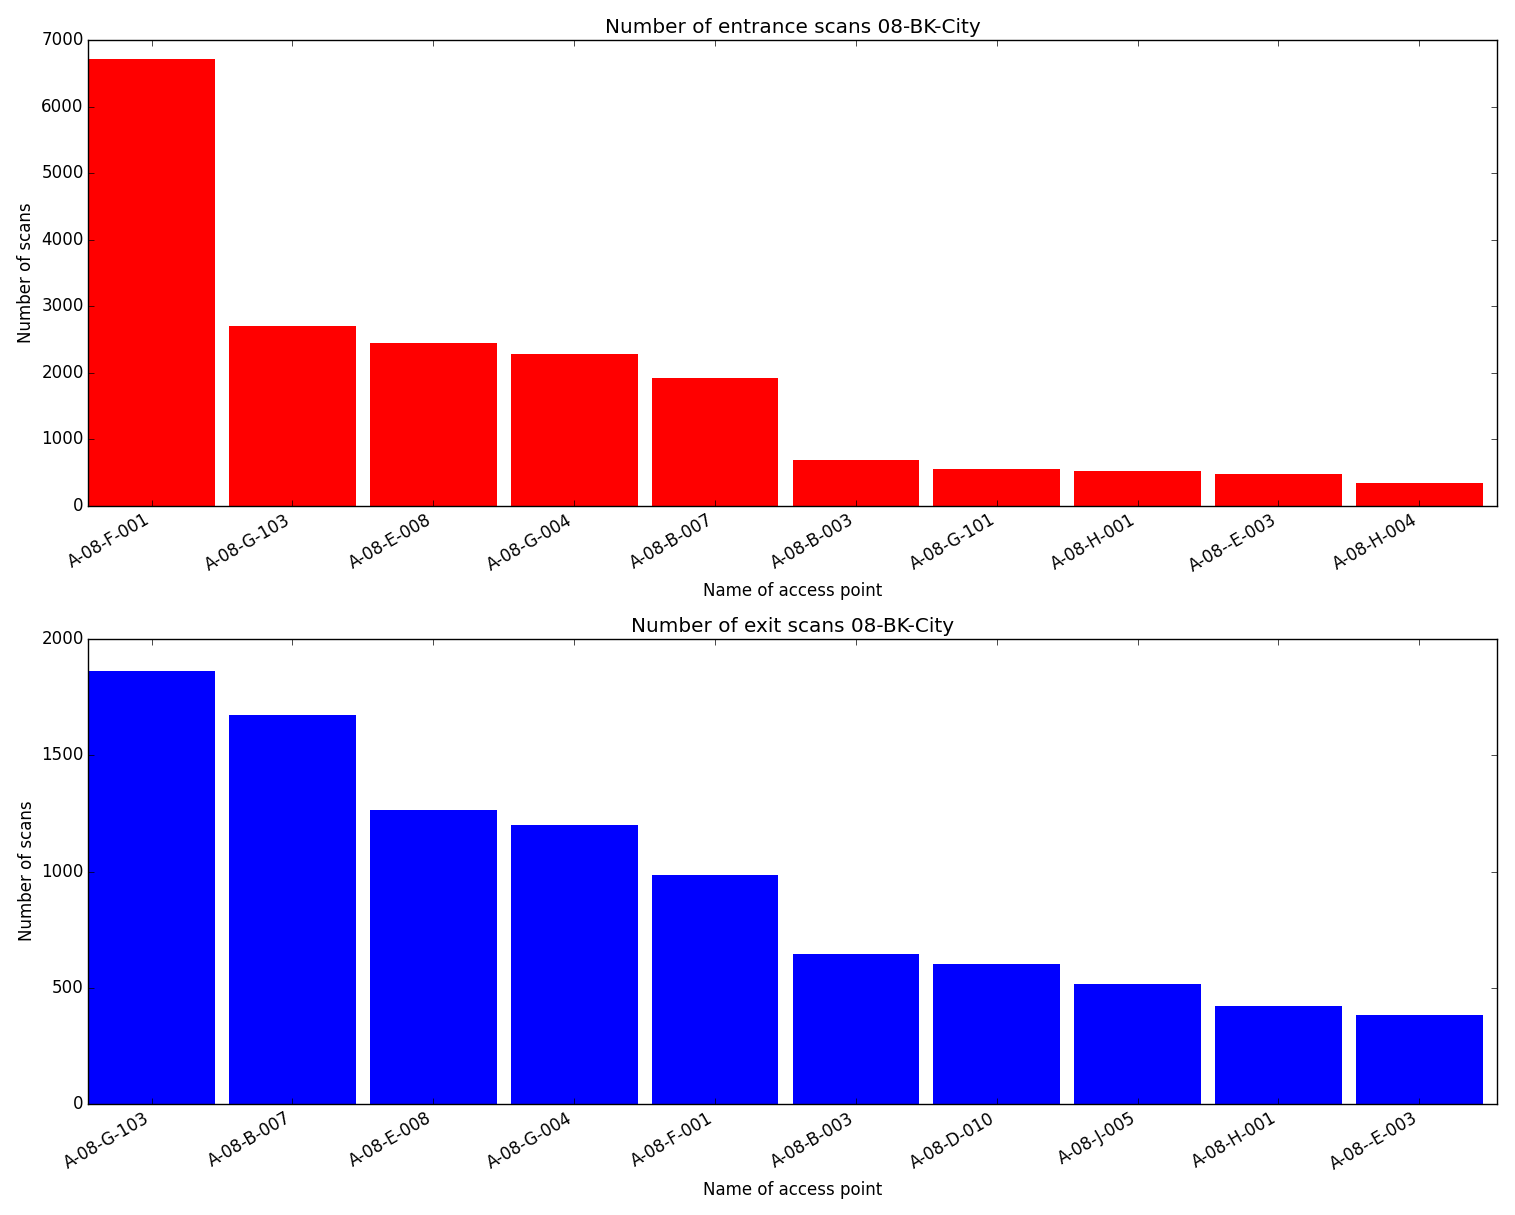
\includegraphics[scale=0.25]{entrances_firstapproach}
\captionsetup{justification=centering}
\caption{Most frequently used entrance and exit access points in BK-City}
\label{figure:Entrance1Approachfigure}
\end{figure}

In order to know whether these access points(see \autoref{figure:Entrance1Approachfigure}) are located near an entrance, the access point maps of BK-City is used. The access point maps are the building plans enriched with the location of each wifi access point installed in the building. Currently, the access point maps of BK-City are the only ones available. Looking at the location of the access points with the highest frequency, gives an interesting result (\autoref{figure:Entrance1Approachaploc}).
 
\begin{figure}[H]
\centering
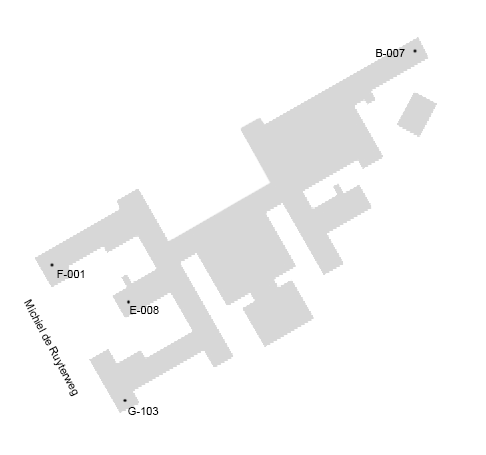
\includegraphics[scale=0.7]{entrances_aplocs_firstapproach}
\captionsetup{justification=centering}
\caption{The location of the most frequently used entrance and exit access points}
\label{figure:Entrance1Approachaploc}
\end{figure}
Most of the frequently used access points are located at the western part of BK-City (\autoref{figure:Entrance1Approachaploc}). Also, there is no entrance or exit located near most of these access points. Knowing that lots of people are passing in the street next to the western part of the building, we can conclude the result of this analysis is distorted due not filtering out the devices that get scanned when passing by the building.

\subsection{Second approach:excluding devices passing by}\label{secondapproach}

\autoref{figure:Entrance2Approachtable} depicts the table as a result of the pre-processing as described in \autoref{preprocessing}. The records represent the stays for each mac, including the first and last access points (ap\_ start and ap\_ end).

\begin{figure}[H]
\centering
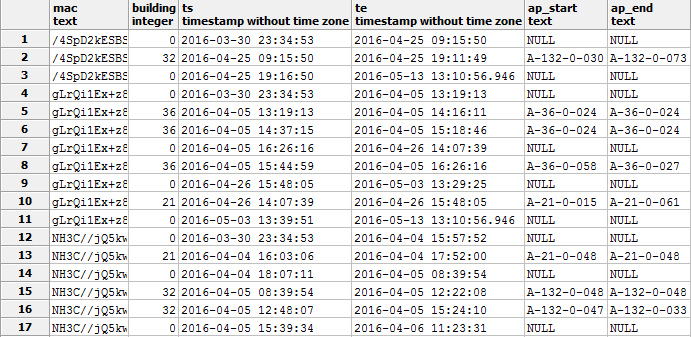
\includegraphics[scale=0.6]{entrances_secondapproach_table}
\captionsetup{justification=centering}
\caption{A segment of the table as a result of the pre-processing}
\label{figure:Entrance2Approachtable}
\end{figure}

The table also includes 'world' (in the \autoref{figure:Entrance2Approachtable} represented by NULL) which implies the device is not located on the campus. 

The following simple SQL statement is used to plots the most frequently used entrance access points.

\begin{lstlisting}[language=SQL]
SELECT ap_start, count(*)
FROM table
GROUP BY ap_start
ORDER BY count desc;
\end{lstlisting}	

Ap\_ end is used, instead of ap\_ start, for plotting the most frequently used exit access points in a building.

\begin{figure}[H]
\centering
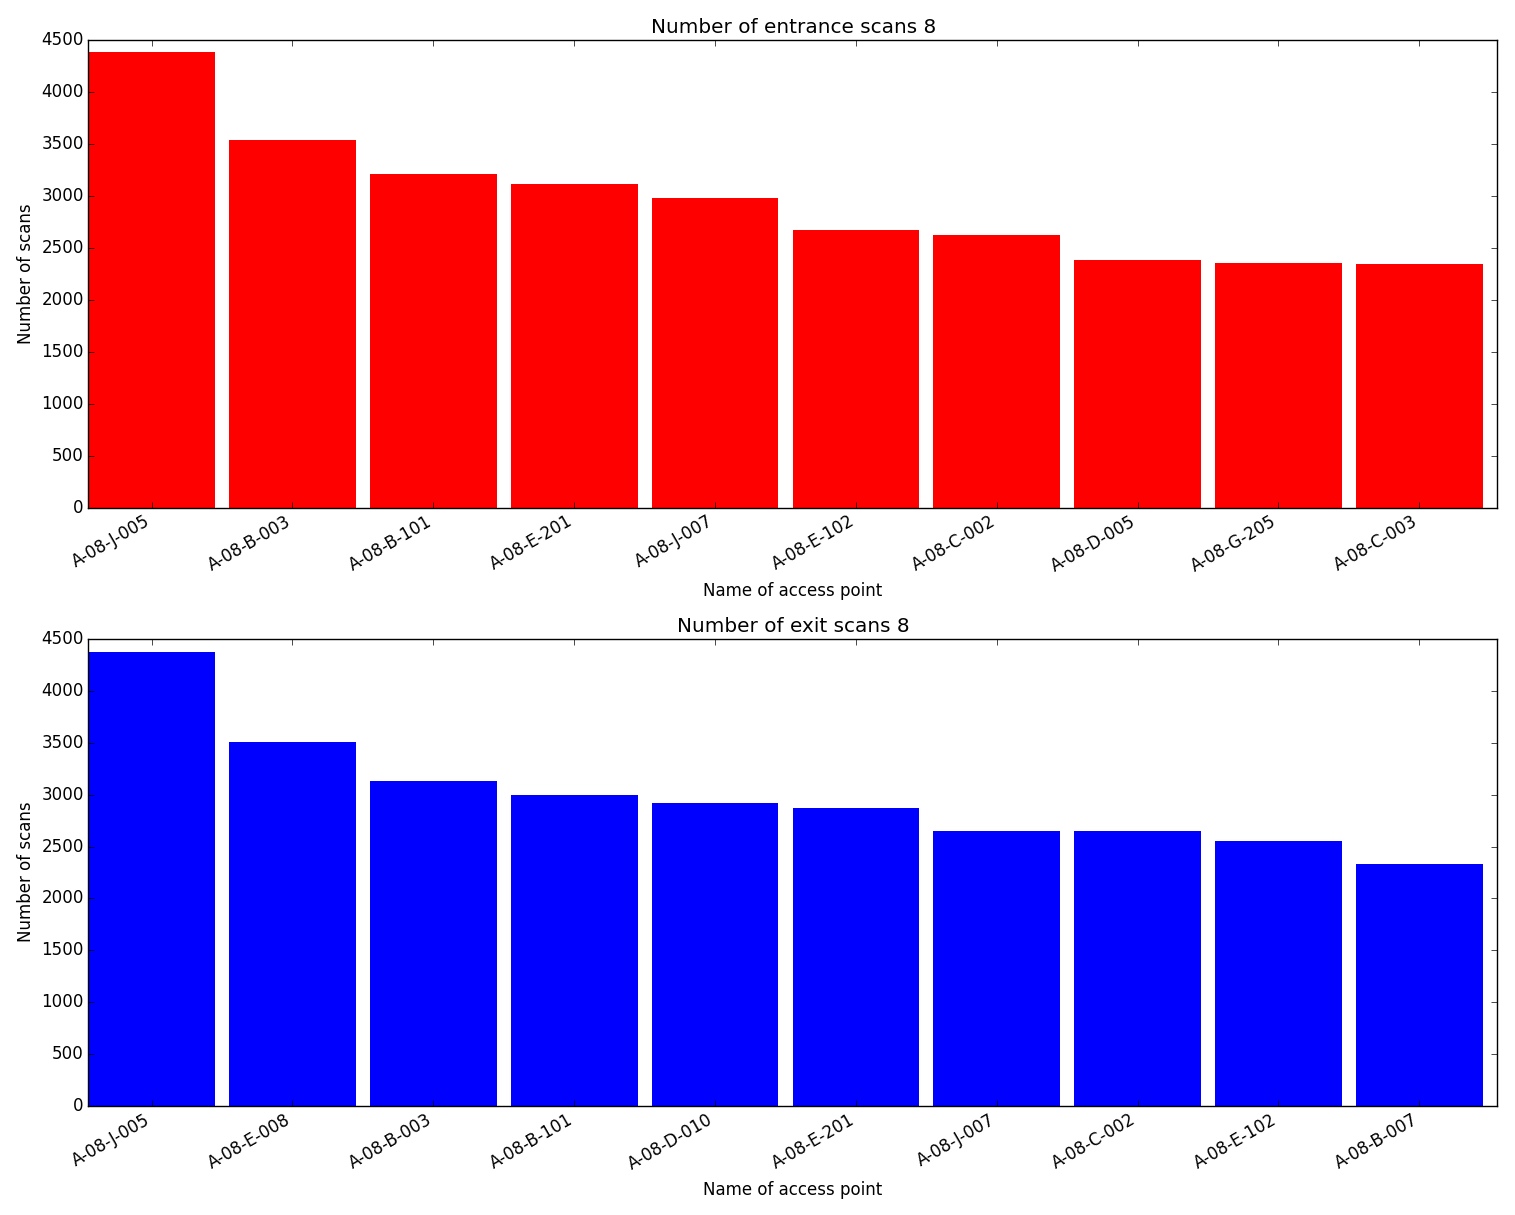
\includegraphics[scale=0.32]{entrances_secondapproach}
\captionsetup{justification=centering}
\caption{The most frequently used entrance and exit access point for BK-City
}
\label{figure:Entrance2Approach}
\end{figure}

The most frequently used access point, A-08-J-005, is not located near an entrance or exit (see \autoref{figure:Entrance2Approach}). This is different than expected. Although it is not very logical in the first place, it still might be one of the first or last access points a device connects with. The reason for this is that the A-08-J-005 access point is placed in in an open space without many objects that could block the wifi signals.

\begin{figure}[H]
\centering
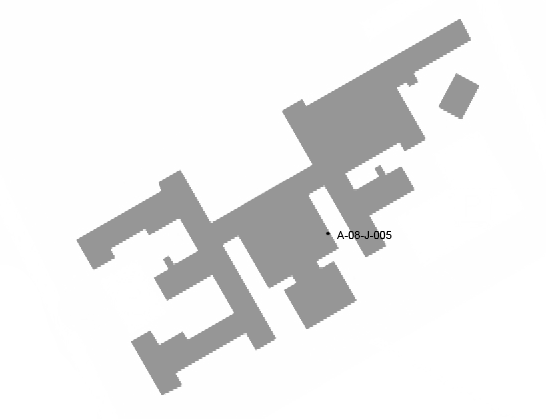
\includegraphics[scale=0.6]{map_ap1_secondapproach}
\captionsetup{justification=centering}
\caption{The location of the most frequently used entrance and exit access point, according to our second approach
}
\label{figure:Entrance2Approachaploc}
\end{figure}

We expected the access point to be located much closer to an entrance or exit. The plan is to set up an experiment in order to justify the unexpected result. In this experiment we will check to what access points different devices (laptops and mobile phones) connect when entering or leaving a building.

\subsection{Frequency of entrance and exit access points}
This section will describe the analysis on the frequency of entrance and exit access points. As described in \autoref{secondapproach}, the most frequently used entrance and exit access points are not always are located near an entrance or exit. Though it is still possible to analyze how frequent these access point are used. The results will be aggregated, meaning it represents more than a single day.

\textbf{Entering}
First we will take a closer look at an access point which appears to be one of the first that scans the device. This will be A-08-J-005 in BK-City, see \autoref{figure:Entrance2Approach} in \autoref{secondapproach}. The chart below shows the frequency of entrance access point A-08-J-005 for devices entering BK-city, over a 24 hour time period. 

\begin{figure}[H]
\centering
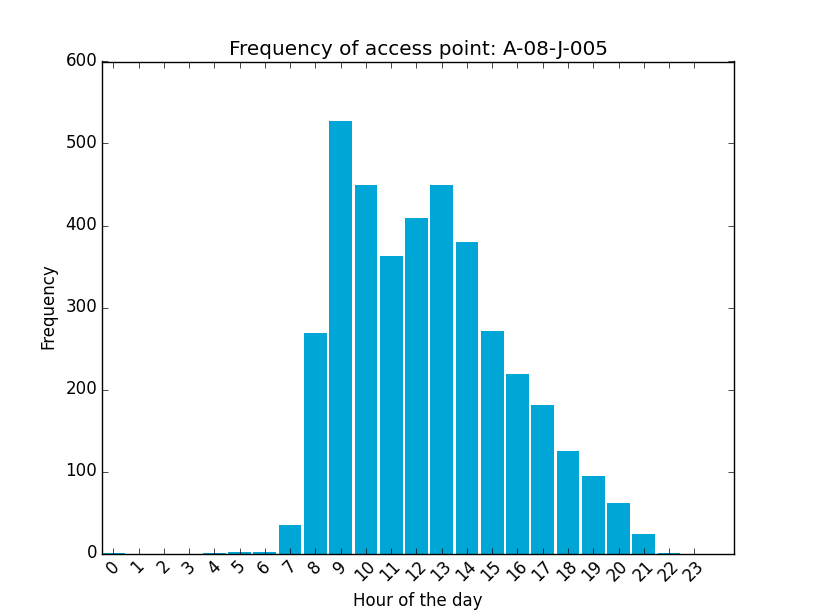
\includegraphics[scale=0.5]{entrances_frequency_secondapproach}
\captionsetup{justification=centering}
\caption{Frequency of entrance access point A-08-J-005
}
\label{figure:A-08-J-005Entrance}
\end{figure}

The chart shows two peaks; in the morning and around 12pm to 1pm. This is in line with what we expected. In the morning a large group enters the building and around 12pm to 1 pm a large group enters the building after the lunch break. 

\textbf{Exiting}

For the exit situation, again the A-08-J-005 access point will be used. This access point also appears to be the most frequently used exit access points. The chart below depicts the frequency of devices leaving the building over a 24 hour period.

\begin{figure}[H]
\centering
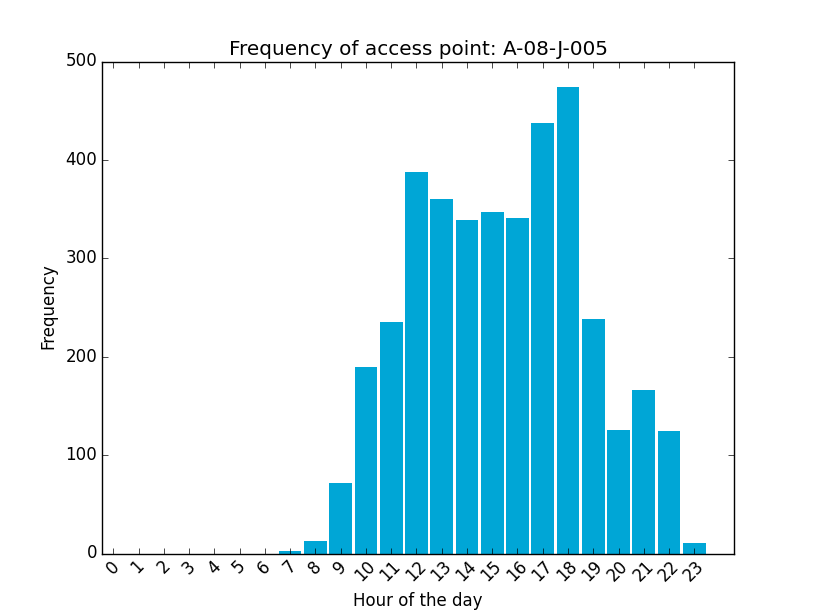
\includegraphics[scale=0.5]{exits_frequency_secondapproach}
\captionsetup{justification=centering}
\caption{Frequency of entrance access point A-08-J-005
}
\label{figure:A-08-J-005Exit}
\end{figure}

The chart shows three interesting peaks, which is in line with what we expected. The first one, around 12am to 1pm, is due to people that leave the building, most probably for lunch. The second peak, around 6pm to 7pm, is due to people that go home for diner. The last one, around 9pm to 10pm, is due to the closing time of the building.

\section{Static and mobile devices}\label{Static and mobile devices}

In order to identify the movement patterns and know what entrances and exits are most frequently used even better, we aim to identify dynamic and static devices. In our first approach, we will look at the number of different access points the device is scanned by in time. The distinction between static and dynamic devices is important, because the behaviour, in terms of Wi-Fi tracking, is significantly different. For instance, a static device, such as a laptop, connects with the Wi-Fi network at different moments compared to a dynamic device, such as a mobile phone. The difference will be explained more in detail using the image below. 

Assume a person that carries a static device (laptop) and a dynamic device (mobile phone) enters a building. While being on his way to the destination, the person does not make use of the laptop, thus the laptop is not connected to the Wi-Fi network. On the other hand, the Wi-Fi of the mobile phone is turned on all the time, and connects at the moment the device is on range of the first access point. On the way the mobile phone is scanned by Access Point(AP) 1, 2 and 3. The person connects to the Wi-Fi network with the laptop at the moment it arrives in the room, of which the Wi-Fi is covered by AP 3. This access point scans the laptop for first time after entering the building. The static laptop is distorting the result, due the fact that in this case the entrance access point for the laptop would be AP 3. In order to achieve a more reliable result, the aim is to filter out the static devices.

To identify the static and dynamic devices, we analyze the behaviour of each device. The first approach focuses on the number of (distinct) access points and the session duration. We assume to find differences between them (\autoref{table:staticanddynamic}). 

\begin{table}[H]
\centering
\begin{tabular}{|c|c|c|}
\hline 
 & Session duration & Nr.of access points \\
\hline
Static & long & low \\
\hline
Dynamic & short & high \\
\hline	
\end{tabular}
\captionsetup{justification=centering}
\caption{Difference between static and dynamic devices}
\label{table:staticanddynamic}
\end{table}

We expect that the relation between the distinct access points and the (summed) session duration, called ratio, is going to be useful in making the distinction between static and dynamic devices (\autoref{equation:staticdynamic}).

\begin{equation}\label{equation:staticdynamic}
Ratio = distinct access point / summed session duration
\end{equation}

In this, a small ratio indicates the device is dynamic and a large ratio indicates the device is static. The result shows that the number of devices decreases over ratio(\autoref{figure:staticanddynamic}).
\begin{figure}[H]
\centering
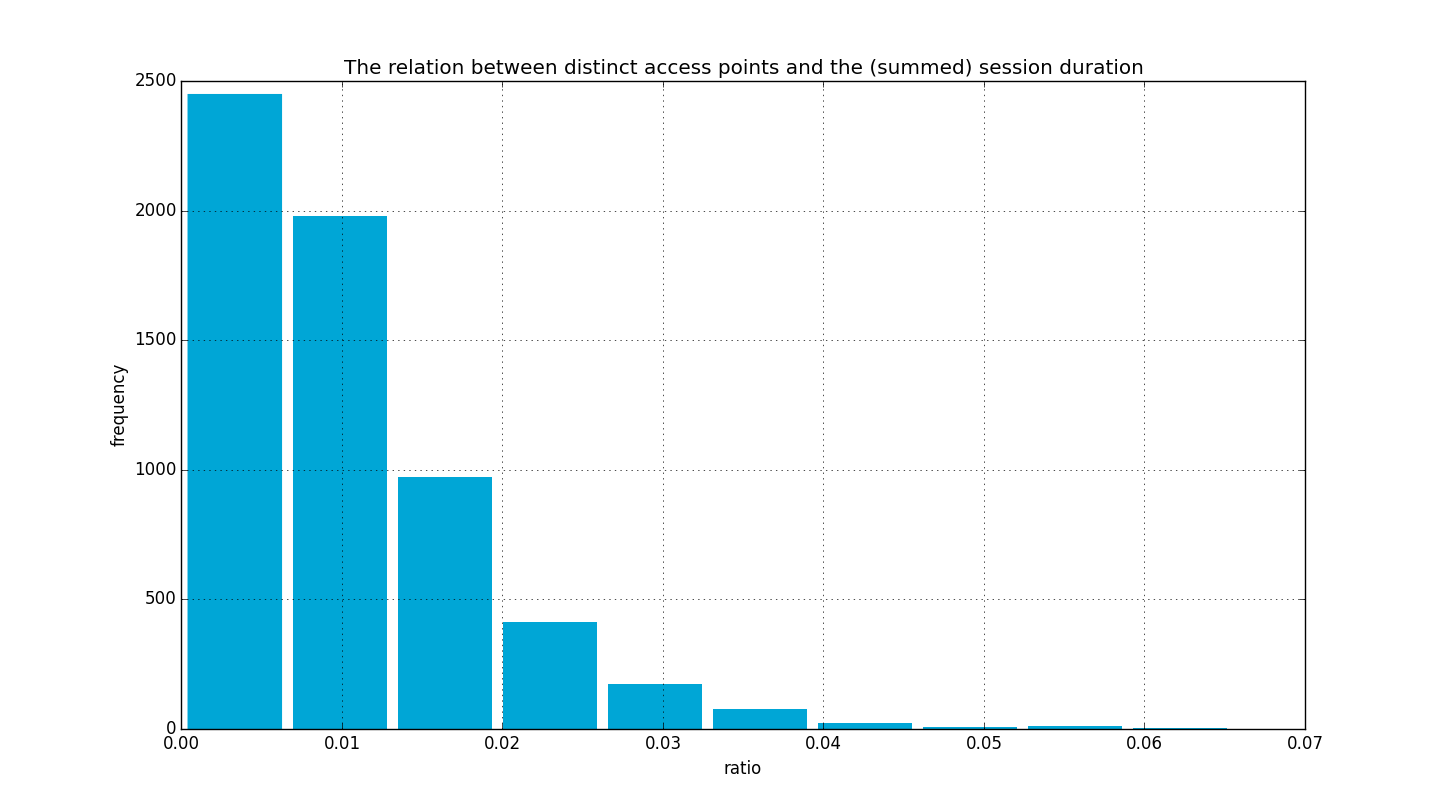
\includegraphics[scale=0.4]{static_vs_dynamic_histogram}
\captionsetup{justification=centering}
\caption{The relation indicating frequency of a radio}
\label{figure:staticanddynamic}
\end{figure}

Because the frequency decreases gradually, there is a fuzzy boundary that separates the static from dynamic devices. Therefore it not (yet) possible to filter out the static devices for further analysis. In order to improve this, the plan is to use the exact number of access points that scanned the device instead of the distinct access points. Also, a closer look will be taken at the session duration, since dynamic devices will have session duration of approximately 5 minutes much more often. 


\section{Preliminary Results}\label{results}

The movement trajectories and the amount of movement between buildings can be visualized in maps and bar charts. The previous sections explained how the data is transformed and this section focusses on the results that can be derived from this data. Bart Valks and Iljoesja Berdrowski stated some questions that arise in their line of work and this section will try to answer these questions with the visualization in both maps and bar charts.
\\\\
\subsection{Movement to the Aula on weekdays}

The department of FMRE would like to know if the faculty of Applied Sciences uses the restaurant facilities of the Aula more than other buildings, due to the fact that the two buildings are connected with a bridge on the first floor.

The graph below shows the average movement of people to the Aula on weekdays. Clearly a peak can be distinguished in the morning between 8:00 and 9:00, around lunch time and in the afternoon between 17:00 and 18:00. The morning and afternoon movements represent people moving from home to the aula and back home.
\begin{figure}[H]
\centering
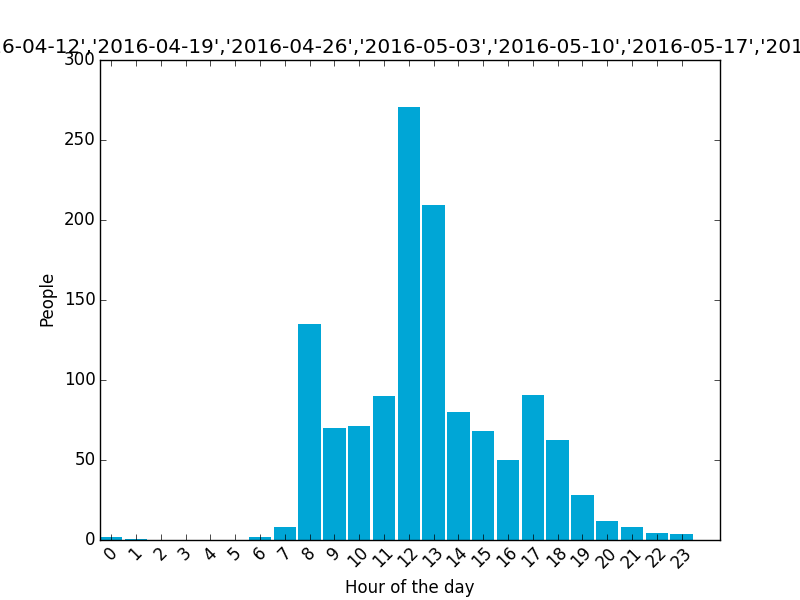
\includegraphics[scale=0.6]{all_to_aula.png}
\captionsetup{justification=centering}
\caption{All to Aula}
\label{figure:all to aula}
\end{figure}

The graph however, says nothing about which buildings contribute the most to the movement to the aula. The map image below shows the top 10 buildings with movement to the aula. It is clear that most of the movement comes from the Library. But if leaving the Library out of the equation, it is clear to conclude that the faculty of Applied Sciences uses the aula more than other faculties. The movement from TNW to the aula is 5000 people over the whole dataset, where other faculties don’t get higher amounts than 2500. 

\begin{figure}[H]
\centering
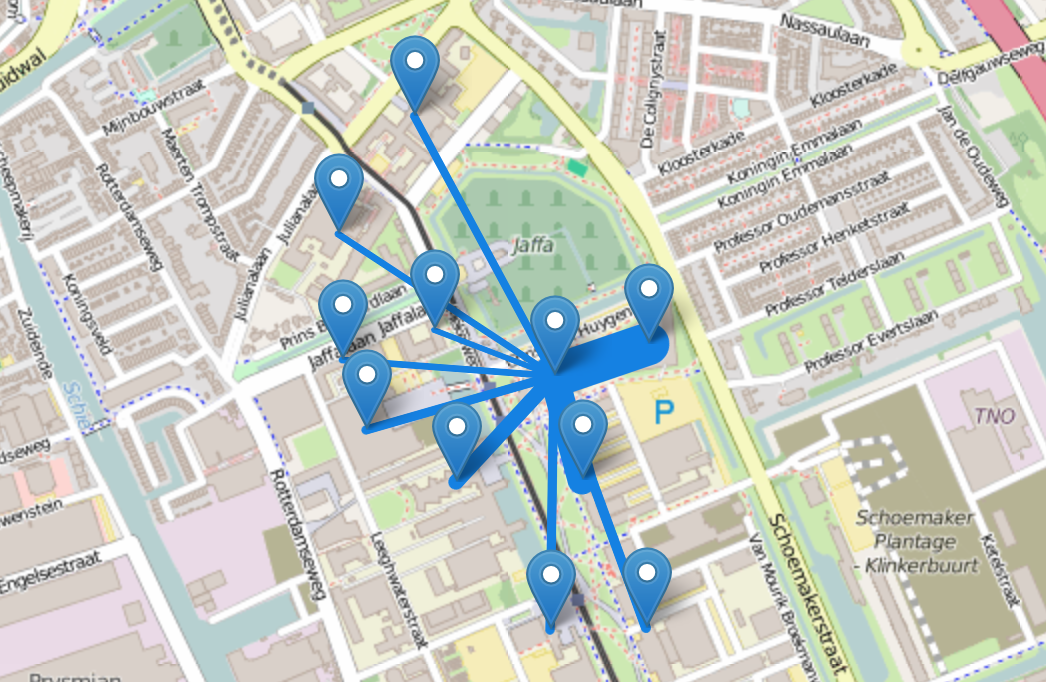
\includegraphics[scale=0.65]{map_all_to_aula.png}
\captionsetup{justification=centering}
\caption{Maps from all buildings to Aula}
\label{figure:all to aula maps}
\end{figure}

This partly confirms the assumption that FMRE made, but to be sure, the movement from the faculty of Applied Sciences must also be checked, in order to see if the movement to the aula is no exception. The result of this visualization is shown in the map image below.

\begin{figure}[H]
\centering
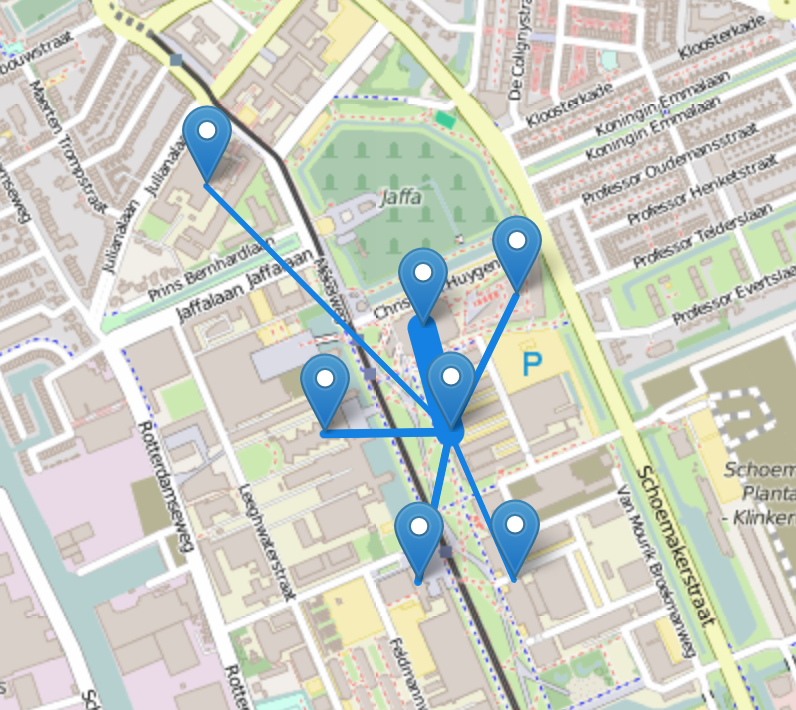
\includegraphics[scale=0.7]{map_all_to_tnw.png}
\captionsetup{justification=centering}
\caption{Maps from all buildings to TNW}
\label{figure:all to TNW maps}
\end{figure} 

This image shows that indeed most of the movement originating from the faculty of Applied Sciences is going to the Aula. The bar chart provides more insight in when this movement is taking place, which is during lunch, as expected. 
\\\\
\subsection{Movement on weekdays vs. weekends}
\begin{figure}[H]
	\centering
	\captionsetup[subfigure]{justification=centering}
	\begin{subfigure}[t]{0.48\textwidth}
	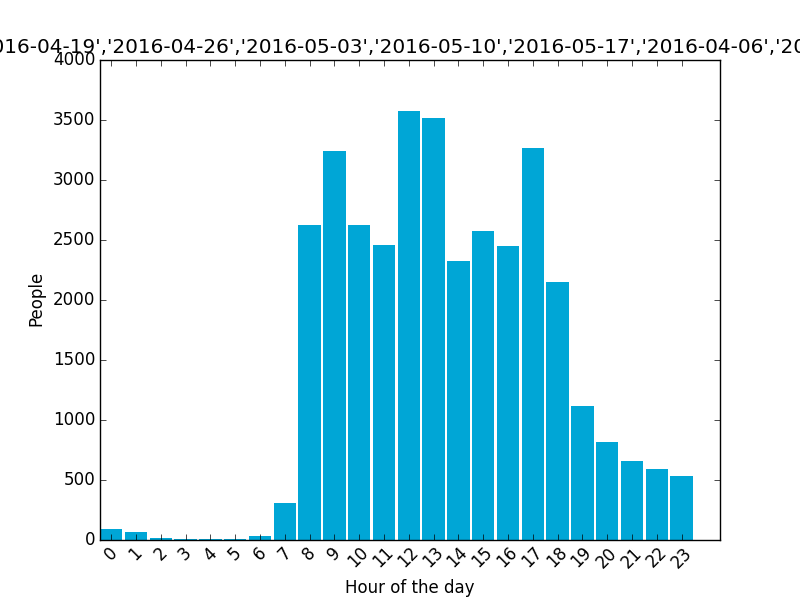
\includegraphics[scale=0.45]{12_weekdays}
	\caption{Movements on weekdays}
	\label{figure:weekdays}
	\end{subfigure}
	\begin{subfigure}[t]{0.48\textwidth}
	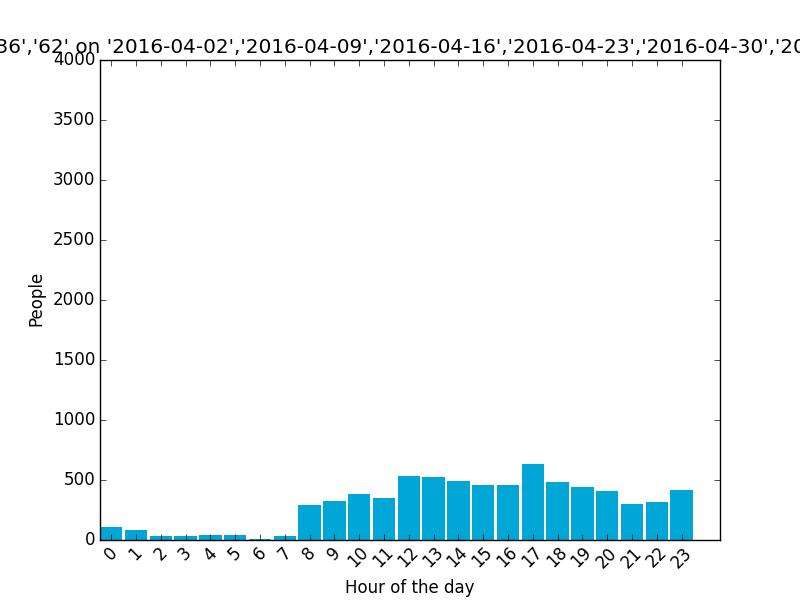
\includegraphics[scale=0.45]{12_weekends}
	\caption{Movement on weekends}
	\label{figure:weekends}
	\end{subfigure}
	\captionsetup{justification=centering}
	\caption{Bar charts of the movements}
\end{figure}

The figures above show the movement from and to the 12 most used buildings on campus. \autoref{figure:weekdays} shows the barplot for the weekdays, \autoref{figure:weekends} shows the barplot for the weekends. It is clear to see that during weekends, there is a lot less movement during weekends. Especially during lunchtime, we can see a peak during weekdays and in the morning and afternoon. In the weekend the movement to the faculties is apparently much less and more spread out over the day.\\
Interesting to see is the movement in the early morning, between 00:00 and 4:00. The library is only open from 8:00 to 2:00, but the bar chart alone does not provide enough information to draw conclusions about these movements.\\\\
\begin{figure}[H]
	\captionsetup[subfigure]{justification=centering}
	\begin{subfigure}[t]{0.48\textwidth}
	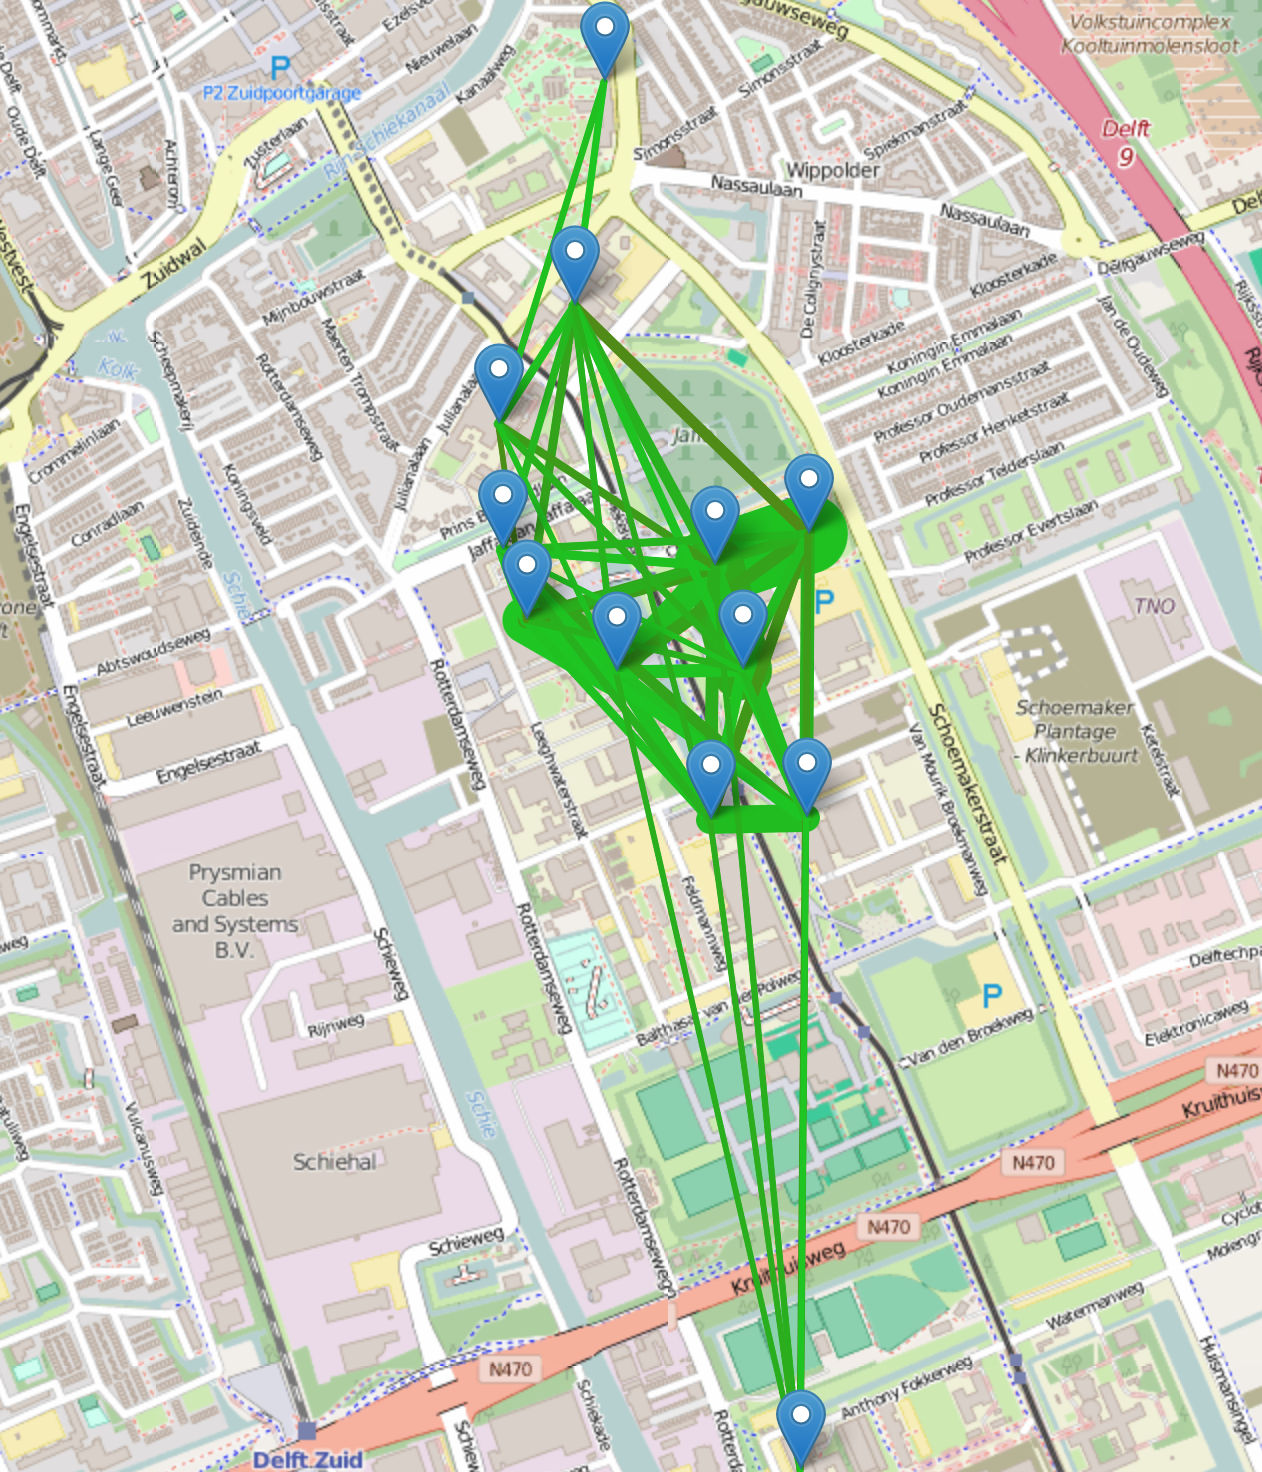
\includegraphics[scale=0.4]{12_weekdays_map}
	\caption{Movements on weekdays}
	\label{figure:map_weekdays}
	\end{subfigure}
	\begin{subfigure}[t]{0.48\textwidth}
	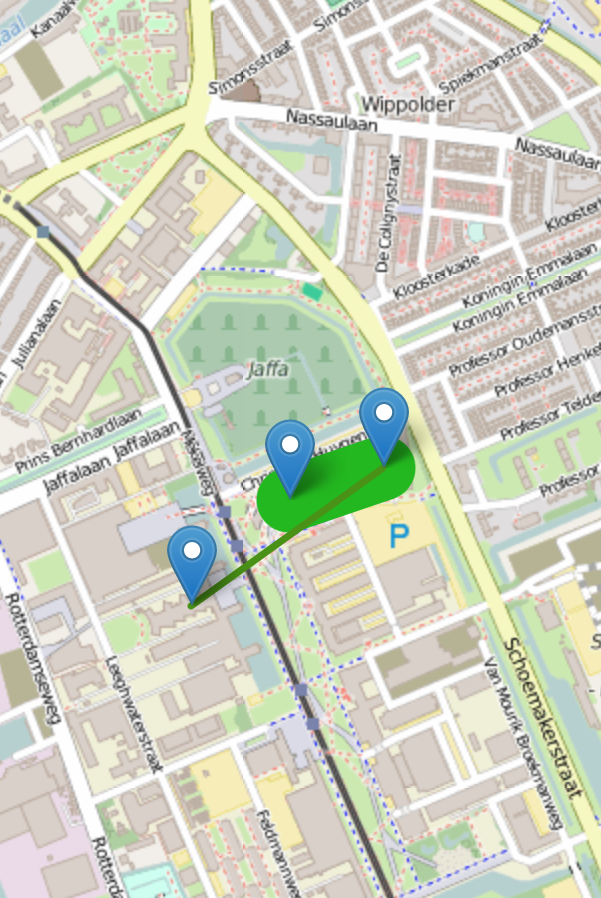
\includegraphics[scale=0.65]{12_weekends_map}
	\caption{Movements on weekends}
	\label{figure:map_weekends}
	\end{subfigure}
	\captionsetup{justification=centering}
	\caption{Maps of the movements}
\end{figure}
\autoref{figure:map_weekdays} and \autoref{figure:map_weekends} show the spread of the movement over the whole campus. Now it becomes clear that movement during weekdays is spread out over all faculties, but during weekends is only focused on the Library. There is however one exception, the faculty of 3ME. This could be explained by staff using the building with their campus card. \\

It is interesting to see that during weekdays the movement from and to a faculty is almost always symmetric, whereas in weekends this is certainly not the case. 

\subsection{Architecture as an island}
The department of FMRE also assume that architecture students and staff have the tendency to stay in their faculty and move less to other buildings on campus than other faculties. \\
Their question can be answered when looking at the movement between the faculty of architecture and all other buildings. This shows the amount of movement to other faculties, but these amounts need to be compared to the movement from other faculties (for this question IO, CiTG and LR are considered) to other buildings. \\

\begin{figure}[H]
\centering
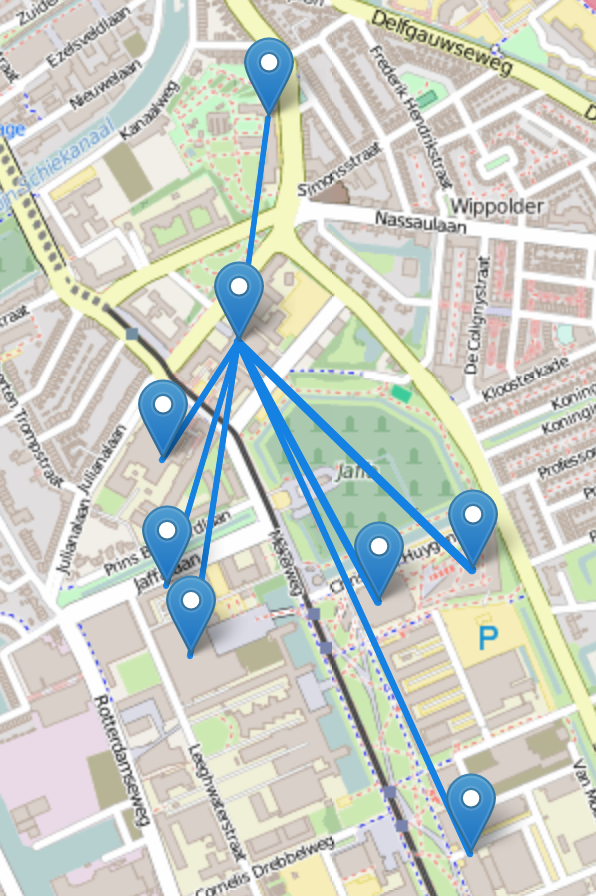
\includegraphics[scale=0.6]{bk_movement_map}
\captionsetup{justification=centering}
\caption{Movement from the faculty of Architecture}
\label{bk_map}
\end{figure} 

\autoref{bk_map} shows the movement between the faculty of architecture and other faculties. The map shows the 7 most used buildings, the movement to other faculties is only 2\% of the total movement and is left out for readability. The total amount of movement from Architecture is 4.239 people. The largest movement to any other faculty is to the Library with 1.043 people. \\

\begin{figure}[H]
\centering
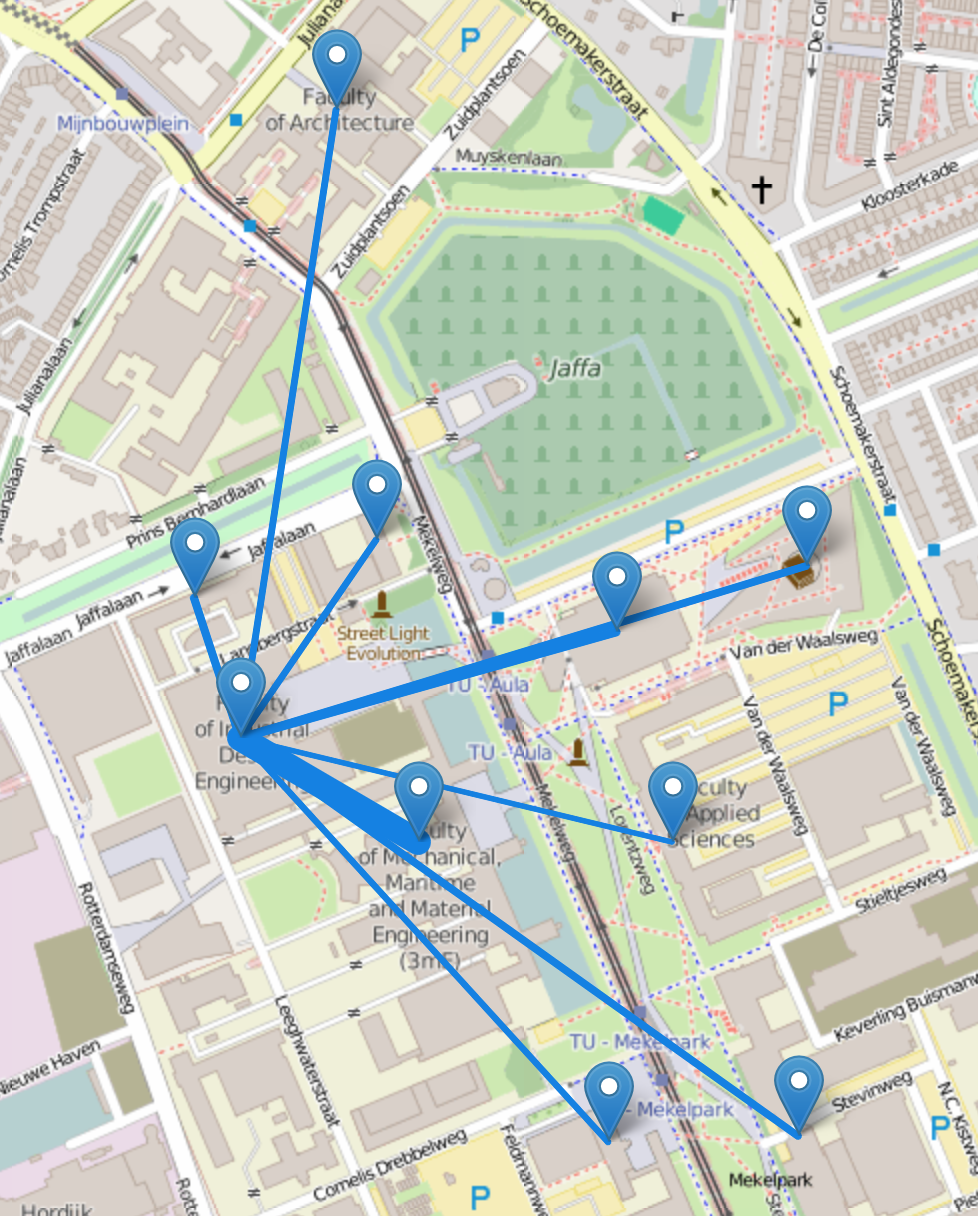
\includegraphics[scale=0.4]{IO_movement_map.png}
\captionsetup{justification=centering}
\caption{Movement from the faculty of Industrial Design}
\label{io_map}
\end{figure} 

\autoref{io_map} shows the movement from the faculty of Industrial Design to other faculties. The total amount of movement from IO is 10.933 people and the biggest movement is to the faculty of 3ME, with 4.927 people. This is already a lot more movement than the faculty of architecture.\\

\begin{figure}[H]
\centering
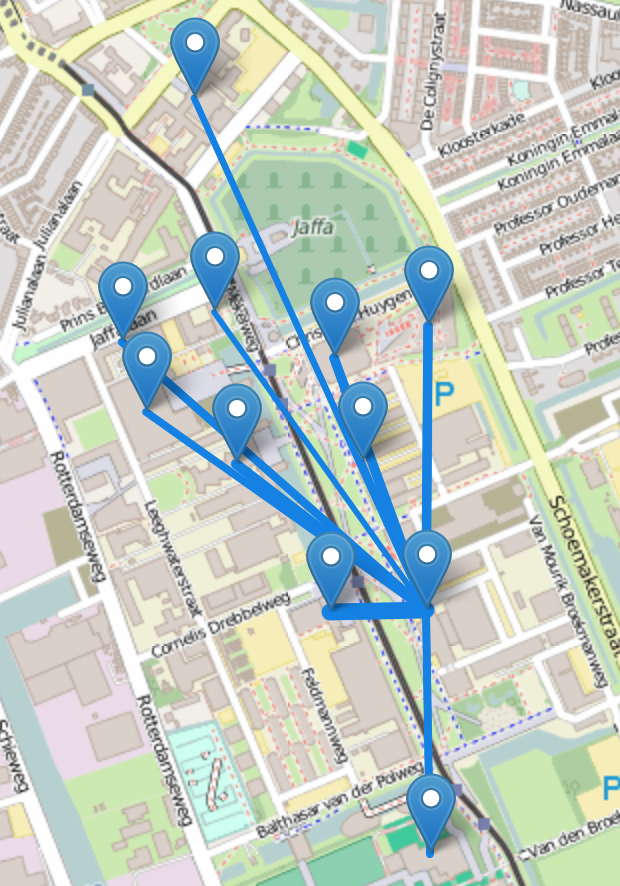
\includegraphics[scale=0.55]{citg_movement_map.png}
\captionsetup{justification=centering}
\caption{Movement from the faculty of Civil Engineering}
\label{citg_map}
\end{figure} 

\autoref{citg_map} shows the movement from the faculty of Civil Engineering to other faculties. The total amount of movement from CiTG is 11.035 people and the biggest movement is to the faculty of EWI, with 2.897 people. This is even more movement than IO.\\

\begin{figure}[H]
\centering
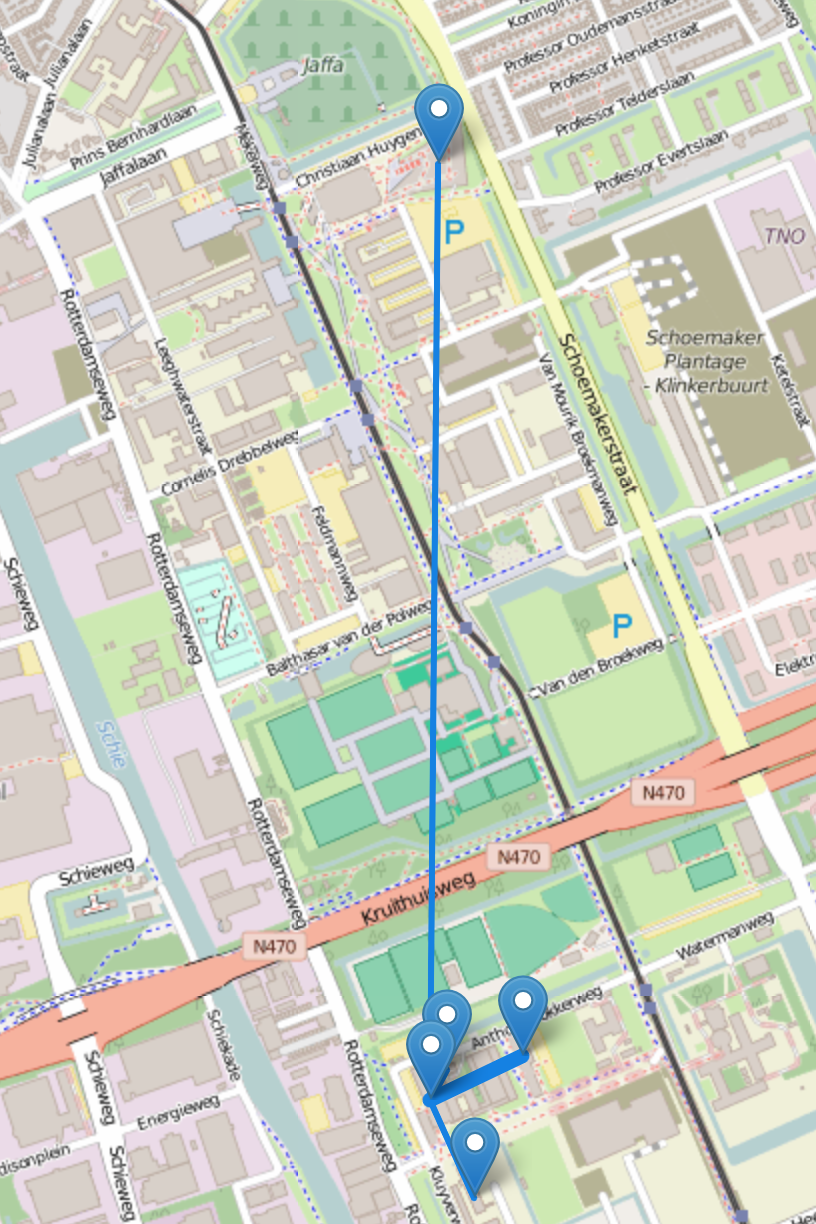
\includegraphics[scale=0.45]{lr_movement_map.png}
\captionsetup{justification=centering}
\caption{Movement from the faculty of Aerospace Engineering}
\label{lr_map}
\end{figure} 

\autoref{lr_map} shows the movement from the faculty of Aerospace Engineering to other faculties. The total amount of movement from AE is 4.348 people and the biggest movement is to the Fellowship, with 2.435 people. 

Looking at these figures we can clearly see that the movement from the faculty of architecture is much less than the movement from Civil Engineering and Industrial Design.  However, the faculty of Aerospace Engineering seems to be even more isolated than architecture. 

\subsection{Movement from and to the campus}
\begin{figure}[H]
\centering
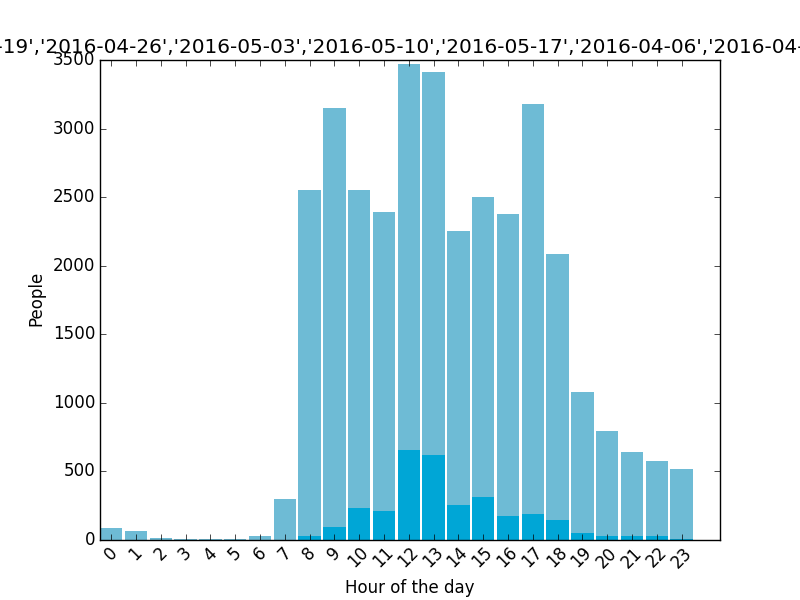
\includegraphics[scale=0.45]{weekdays.png}
\captionsetup{justification=centering}
\caption{Movement from and to the campus}
\label{newWeekdays}
\end{figure} 
The aggregated movement from the different faculties is shown in \autoref{newWeekdays}. For this bar chart, a distinction is made between movement that is either from or to the campus(in light-blue) and movement between buildings on campus (darker blue). This will result in a more accurate visualization of the data.

However, the movement from or to the campus is derived from finding gaps of more than one hour in the data, because devices going offline for more than one hour could be considered moving away from the campus. But this does also include devices that are for some reason turned off for more than one hour, such as laptops during lunch breaks or lectures. For these graphs to really accurately show the movement from and to the campus, devices should be categorized into dynamic devices, such as mobile phones and tablets, and static devices, such as laptops. That way, only the dynamic devices can be considered and the graph would be more realistic.
\\\\
\\\\
\\\\
\\\\
\\\\
\\\\
\pagebreak
\section{Future work}
The following sections describe in detail our plan for the next phase in the Synthesis Project. First, the the updated work packages and sprint targets are described, followed by a Gantt chart. At last the potential risks are estimated and solutions are provided.

\subsection{Updated Project Management Plan}
\textbf{Work Packages and process}

\begin{figure}[H]
\centering
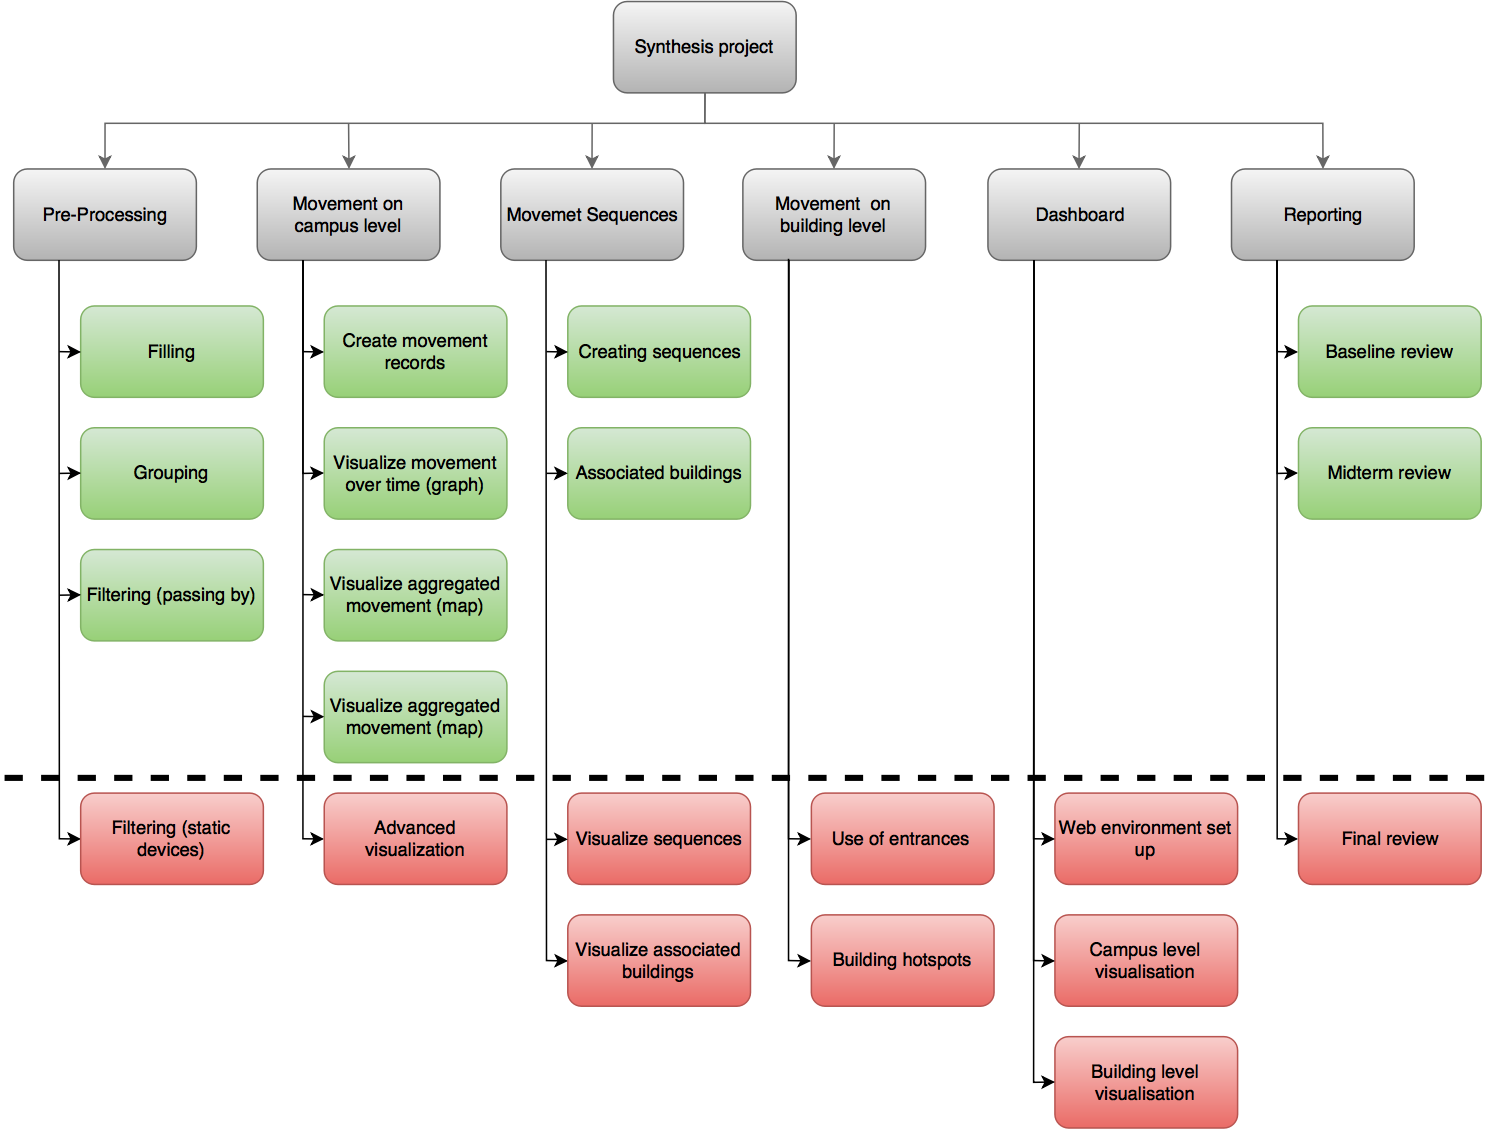
\includegraphics[scale=0.15]{WBS_MidTerm.png}
\captionsetup{justification=centering}
\caption{Updated Work Breakdown Structure}
\label{wbs_MT}
\end{figure} 

\autoref{wbs_MT} displays the completed work packages (green) and the remaining work packages (red).

\textbf{Pre-Processing / Filtering static devices}\\
Stationary and mobile devices are differentiated in the data and the stationary devices are filtered out.\\
\textit{Outcome:} Wi-Fi-log dataset that does not contain stationary Wi-Fi devices.

\textbf{Movement on campus level / Use of entrances}\\
Which BK-City entrances are used when arriving/going to a specific building? How does the use of the entrances of the BK-City change throughout the day, week?\\
\textit{Outcome:} The answer to the questions above.

\textbf{Movement on campus level / Advanced visualization}\\
Based on the feedbacks on the previous trajectory visualizations, the methods for visualizing movement patterns and trajectories are finalized.\\
\textit{Outcome:} Visualization methods that produce clear and easily understandable visualizations for movement patterns in a time range, between locations, display the amount of movement, display the use of entrances.

\textbf{Movement sequence mining / Visualize sequences}\\
\textit{Outcome:} Visualization of the directed movement patterns between buildings.

\textbf{Movement sequence mining / Visualize associated buildings}\\
\textit{Outcome:} Visualization of the building groups, that displays which buildings are frequently visited together.

\textbf{Movement on building level / Clustering access points}\\
Cluster access points in the BK-City to identify hotspots in the building. Our knowledge on the use of the building provides verification for the results. \\
\textit{Outcome:} Hotspots in the BK-City.

\textbf{Movement on building level / Creating movement records}\\
Create a dataset for the BK-City that contains the records that represent movement.\\
\textit{Outcome:} Movement patterns in the BK-City.

\textbf{Movement on building level / Visualization}\\
\textit{Outcome:} Visualization of the movement patterns in BK-City, based on the previously identified hotspots.

\textbf{Dashboard / Web environment set up}\\
Set up the web environment for the dashboard.\\
\textit{Outcome:} The web framework and environment that is used by the dashboard.

\textbf{Dashboard / Campus level visualization}\\
\textit{Outcome:} Dashboard visualization of the movement between buildings on the campus.

\textbf{Dashboard / Building level visualization}\\
\textit{Outcome:} Dashboard visualization of the movement in the BK-City.

\textbf{Reporting / Final review}\\
\textit{Outcome:} Final report and presentation.

\subsection{Sprint targets}
\textbf{Week 6}
\begin{itemize}
\item Wi-Fi-log dataset that does not contain stationary Wi-Fi devices.
\item Analysis and visualization of the use of BK-City entrances throughout a day, week.
\item Visualization methods that produce clear and easily understandable visualizations for movement patterns in a time range, between locations, display the amount of movement, display the use of entrances.
\item Visualization of the directed movement patterns between buildings.
\item Visualization of the building groups, that displays which buildings are frequently visited together.
\end{itemize}
\textbf{Week 7}
\begin{itemize}
\item Hotspots in the BK-City.
\item Movement patterns in the BK-City.
\end{itemize}
\textbf{Week 8}
\begin{itemize}
\item Dashboard
\item Final report and presentation.
\end{itemize}

\subsection{Gantt-chart}
\begin{figure}[H]
\centering
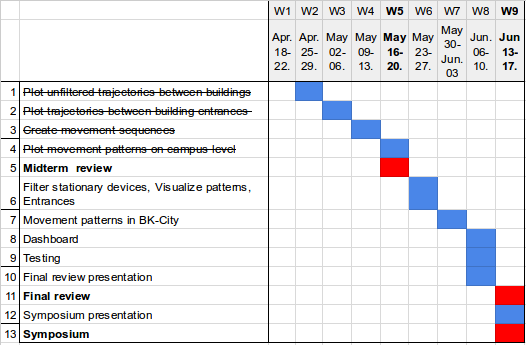
\includegraphics[scale=0.65]{Gantt_2016-05-18.png}
\captionsetup{justification=centering}
\caption{Updated Gantt-chart}
\label{gantt}
\end{figure} 

\autoref{gantt} displays the Gantt-chart of our project.
\pagebreak
\subsection{Risk assessment}
We identified the following risks for the project:
\begin{itemize}
\item Access point map for the whole campus is not available
	\begin{itemize}
	\item \textbf{Solution:} Use only the the access points of BK-City for the analysis
	\end{itemize}
\item We are not able to automatically identify access point clusters (hotspots) in BK-City
	\begin{itemize}
	\item \textbf{Solution:} Refer to our knowledge on the use of the BK-City to manually identify hotspots
	\end{itemize}
\item The visualizations are difficult, unclear to interpret for our client
	\begin{itemize}
	\item \textbf{Solution:} Collect feedback on the intermittent visualizations from multiple sides. Keep our client posted on the results from visualization process.
	\end{itemize}
\item We are not able to identify stationary and moving devices in the data
	\begin{itemize}
	\item {Solution:} Assume a ratio of stationary/moving devices
	\end{itemize}
\end{itemize}
\begin{figure}[H]
\centering
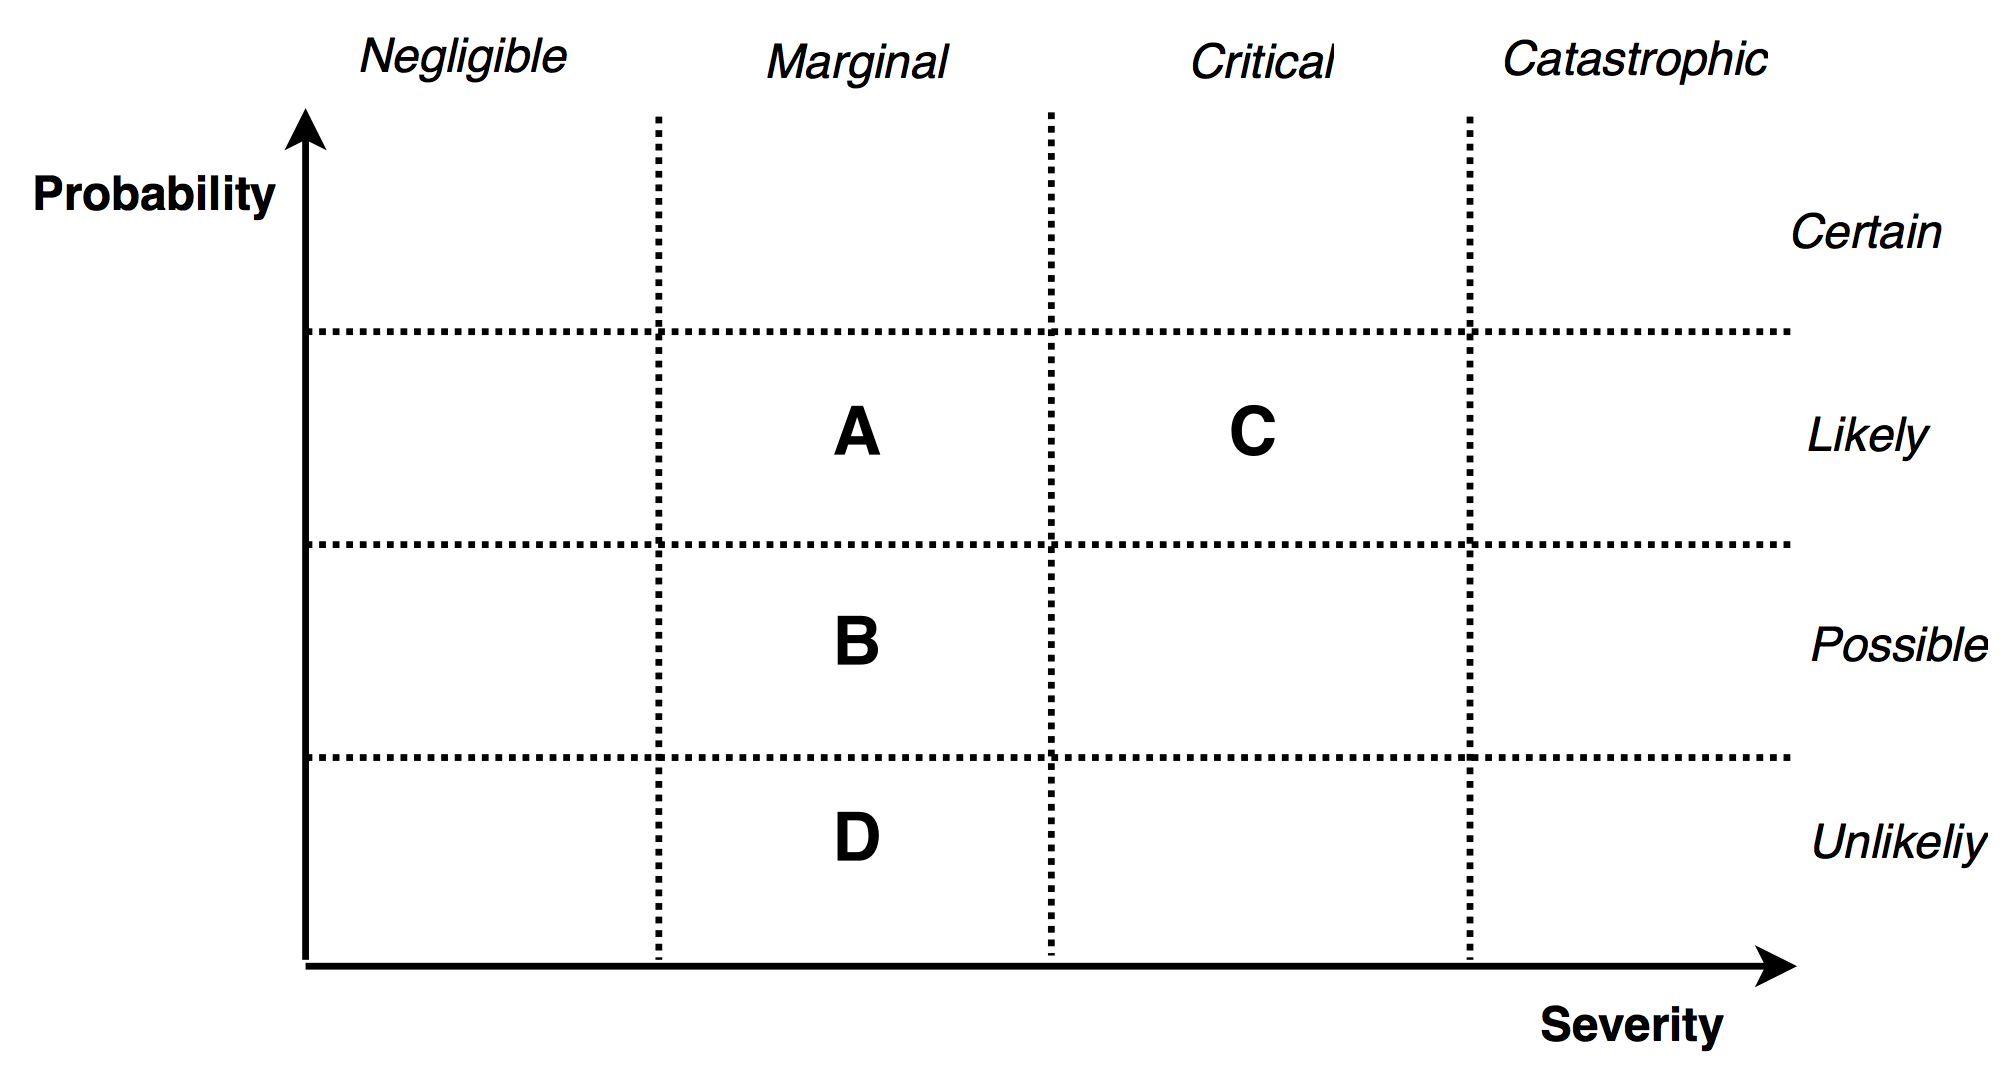
\includegraphics[scale=0.15]{tech_risk_ass.png}
\captionsetup{justification=centering}
\caption{Technical Risk Assessment}
\label{riskass}
\end{figure} 
\autoref{gantt} displays the Gantt-chart of our project.
\autoref{riskass} displays how we evaluated the severity and possibility of each identified risk.
